\documentclass{report}

\usepackage{graphicx}
\usepackage{amsmath}
\usepackage{epstopdf}
\usepackage{url}
\usepackage{verbatimbox}
\usepackage{pdfpages}
\usepackage{supertabular}
\usepackage{footnote}

\DeclareMathOperator*{\argmin}{arg\,min}


\title{\LARGE \bf
A Multiple-Camera System Calibration Toolbox
}

%\author{
%Bo Li \\ Advised by Kevin K\"oser and Marc Pollefeys\\
%Computer Vision and Geometry Group\\ ETH Zurich
%}

\begin{document}

%\maketitle

\begin{titlepage}
\noindent 
\includegraphics[width=0.4\textwidth]{images/ethlogo-print.png}
\vspace*{\fill}
\begin{center}
{\Huge \bf A Multiple-Camera System\\[12pt] Calibration Toolbox}\\[50pt]
{\huge Bo Li}\\[30pt]
\begin{tabular}{cl}
\Large Advisors: & \Large Dr. Kevin K\"oser\\[8pt]
& \Large Prof. Marc Pollefeys
\end{tabular}
\\[100pt]
{\LARGE Master Thesis}\\[25pt]
{\Large Computer Vision and Geometry Group}\\[8pt] 
{\Large Department of Computer Science}\\[8pt]
{\Large ETH Zurich}\\[40pt]
{\Large 2013 May 25}
\end{center}
\vspace*{\fill}
\end{titlepage}

\tableofcontents

\begin{abstract}
This thesis presents some recent developments on camera calibration. It includes the following contents: 

1) An calibration approach for multiple-camera systems. We propose a novel feature descriptor-based calibration pattern. It can be used for easily calibrating both the intrinsics and extrinsics of a multiple-camera system. The calibration only requires that neighboring cameras observe parts of the calibration pattern at the same time; the observed parts may not overlap at all. No overlapping fields of view are assumed for the camera system.

2) An open source multiple-camera system calibration toolbox for Matlab. The proposed toolbox supports the calibration of a camera system which can comprise either normal pinhole cameras or catadioptric cameras. We show that the toolbox can be easily used to automatically calibrate camera systems. 

3) Some explorations on the calibration problem in scenario of camera-display pair. LCD displays are used for displaying a specially designed calibration pattern. We show an experiment of measuring the grayscale response function of the LCD display and propose an approach for refining camera calibration result using the estimated grayscale response function. 


\end{abstract}



\chapter{Introduction}
Multiple-camera systems have become increasingly prevalent in robotics and computer vision research. These systems include mature products e.g. stereo camera or Ladybug camera, and also a large variety of customized camera systems. Commonly used cameras in the systems include normal pinhole cameras, wide-angle cameras and fish-eye cameras. To make such systems to work properly, both the intrinsics and extrinsics of the cameras should be well calibrated. 

\section{Related Work}
Recently, many efficient methods have been developed for intrinsic calibration of many types of cameras. These methods can be divided into two categories: calibration with a special calibration object, and self-calibration. In this paper, we focus on the former category which is usually much more accurate than self-calibration. Many toolboxes are available for this category of methods. Seminal work on calibrating a pinhole camera can be found in \cite{zhang2000flexible}. Some popular calibration toolboxes \cite{bouguet2004camera,stoyanov2006camera, opencv_library} are inspired by this method. For generic cameras, \cite{scaramuzza2006toolbox} proposes a toolbox to use a polynomial to approximate rays corresponding to each image point. This method generically applies to most camera models but does not provide a closed-form solution for undistorting raw images. In the toolbox proposed in \cite{mei2007single}, an unified projection model is proposed for calibrating a catadioptric system, fish-eye camera and sphere mirror system. This model is similar with \cite{scaramuzza2006toolbox} but parameterizes rays instead of using an arbitrary polynomial, which makes undistortion much simpler. Details about the previous intrinsic calibration methods can be found in section \ref{singleSec}. 

Some toolboxes are also available for calibrating some simple multiple-camera systems. \cite{bouguet2004camera, opencv_library} enables one to calibrate a stereo camera. For calibration on a system of more than two cameras, these toolboxes \cite{svoboda2005convenient,easycal} can be used. These calibration toolboxes make use of the overlapping fields of view of the cameras; hence, these toolboxes can calibrate a stereo camera and a circular camera rig with all cameras pointing inwards. However, these toolboxes are not suitable for calibrating a system of cameras with no or minimal overlapping fields of view. There is increasing popularity of the use of a camera rig with cameras pointing outwards in both academia and industry; this system cannot be easily calibrated using existing calibration toolboxes due to the minimal overlapping fields of view. Hand-eye calibration algorithms \cite{tsai1989new,shiu1989calibration} can be used to calibrate this system but requires reconstructing visual odometry for each camera, and the calibration is often not accurate due to visual odometry drift. Details about some existing multiple-camera calibration methods can be found in section \ref{extrinsicSec}. 

In addition to camera models, research has also focused on development of easy-to-use calibration patterns. Early research makes perpendicular planes with chessboard patterns or circular dots on their surfaces \cite{bouguet2004camera}. This calibration object is not very convenient since it is not easy to build perfectly perpendicular planes. Current state-of-art calibration systems mainly make use of calibration boards which are often planes with a chessboard or circular dots printed on them. Automatic detector for such patterns is readily available \cite{opencv_library, rufli2008automatic, geiger2012automatic}. A comparison of calibration accuracy between a chessboard and circular dots can be found in \cite{mallon2007pattern}. One disadvantage of these patterns is that the entire pattern has to be visible in each calibration image; this requirement excludes cameras with minimal overlapping fields of view. In addition to the chessboard and circular dots, some other patterns have been proposed. \cite{schmalz2011camera} uses a temporal coded pattern to calibrate cameras. This method uses the Gray code to match world points and image points, thus not requiring the entire pattern to be in the image. The drawback of this method is the limited flexibility; the calibration requires both a display projector and a tripod for mounting a camera. More details about calibration pattern design can be found in section \ref{patternSec}. 

\section{Motivation}
\label{motiveSec}
Existing calibration toolboxes using the chessboard and circular-dot patterns offer ease-of-use and high calibration accuracy when it comes to calibrating single and stereo cameras. However, for a system with multiple cameras pointing in different directions, it is difficult to use these toolboxes to calibrate the extrinsics of the camera system. This is because current automatic and semi-automatic chessboard detectors require the chessboard to be entirely within the field of view of the cameras. Therefore, if two cameras have minimal overlapping field of view, it is difficult to use the chessboard for extrinsic calibration in contrast to stereo camera calibration. The extrinsic calibration for cameras with minimal overlapping fields of view can be made easier if we relax the requirement that the calibration pattern be seen in its entirety by each camera; ideally, the calibration board is automatically detected even when the cameras observe different parts of the board. For most multiple-camera systems, it is fairly common for a camera pair to see different parts of a suitably-sized calibration board at the same time. Based on this motivation, we design a feature descriptor-based calibration pattern which is easy to detect even when seen partially by a camera, and a extrinsic calibration framework using this pattern. 



\section{Contributions}

The main part of this thesis makes two novel contributions: 

\begin{enumerate}
\item A new calibration pattern that encodes feature points using feature extraction techniques. Our pattern contains a large number of detectable features on multiple scales, as illustrated in chapter \ref{patternSec}. The pattern can be recognized and localized even if the pattern is partially seen in an image. 
\item A toolbox based on the proposed calibration pattern. This toolbox can be used for both intrinsic and extrinsic calibration of a multiple-camera system, as illustrated in chapters \ref{singleSec} and \ref{extrinsicSec}. Similarly to existing calibration toolboxes, our toolbox can also be used for intrinsic calibration of a single camera. 
\end{enumerate}

\chapter{Notations}
\begin{supertabular}{p{0.3\textwidth}p{0.67\textwidth}}
$\mathbf{A} \sim \mathbf{B}$ & Vector $\mathbf{A}$ has the same direction with vector $\mathbf{B}$. $\mathbf{A} = \mu \mathbf{B}$, with $\mu$ as some unknown scale factor.  \\[8pt]
$\mathbf{A} \times \mathbf{B}$ & Cross product \\[8pt]
\hline\\[4pt]
$\mathbf{X}^w = [X^w, Y^w, Z^w]^\top$ & A 3D point in the world coordinate system, in the homogeneous coordinate form.\\[8pt]
$\mathbf{X}^c = [X^c, Y^c, Y^c]^\top$ & A 3D point in the camera coordinate system. \\[8pt]
$\mathbf{x} = [x, y]^\top$ & A 2D image point on a normalized image plane with unit focal length. \\[8pt]
$\mathbf{x}' = [x', y']^\top$ & A 2D image point with lens distortion on a normalized image plane with unit focal length. \\[8pt]

$\mathbf{d}_\text{rad} = [dx_\text{rad}, dy_\text{rad}]^\top$ & A image point deviation on the normalized image plane due to the radial lens distortion. \\[8pt]
$\mathbf{d}_\text{tan} = [dx_\text{tan}, dy_\text{tan}]^\top$ & A image point deviation on the normalized image plane due to the radial lens distortion. \\[8pt]
$\mathbf{m} = [u, v]^\top$ & A image point in pixel. \\[8pt]
$\gamma_1$, $\gamma_2$, $\gamma$ & The focal length of the camera. \\[8pt]
$[u_0, v_0]^\top$ & The principal point of the camera in pixel. \\[8pt]
$k_1, k_2, p_1, p_2$ & The radial and tangent lens distortion coefficients. \\[8pt]
$\phi$ & The incident angle between the light ray and the optical axis. \\[8pt]
$\xi$ & The distortion parameter related with the camera type in the catadioptric camera model. \\[8pt]
$\mathbf{K}$ & The intrinsic matrix for the camera. \\[8pt]
$\mathbf{R}$, $\mathbf{t}$ & The rotation and translation from the world coordinate system to the camera coordinate system. \\[8pt]

$\mathbf{p}^w = [X^w, Y^w, 1]^\top$ & The homogenous coordinates of the point $[X^w, Y^w]^\top$ on the calibration pattern plane. This point is denoted as $[X^w, Y^w, 0]^\top$ in the 3D world coordinate system. \\[8pt]
$\mathbf{p}' = [x', y', 1]^\top$ & The homogenous coordinates for point $\mathbf{x}'$. \\[8pt]

$\mathbf{H}$ & A homography between two planes, denoted as a $3\times3$ matrix. \\[8pt]

$\mathcal{P} = 
\begin{bmatrix}
	\begin{array}{cc}
	\mathbf{R} & \mathbf{t}\\
	\mathbf{0} & 1
	\end{array}
\end{bmatrix}$ & A $4\times4$ matrix denoting the pose of the camera or the calibration pattern. \\[8pt]

$\mathcal{C}$ & The set of the intrinsic parameters of a camera. \\[8pt]

$\hat{\mathbf{m}}(\mathbf{X}^w, \mathbf{R}, \mathbf{t}, \mathcal{C})$, $\hat{\mathbf{m}}(\mathbf{X}^w, \mathcal{P}, \mathcal{C})$ & The reprojected image point of the 3D world point $\mathbf{X}^w$, under the given intrinsics $\mathcal{C}$ and extrinsics $\mathcal{P}$ or $\mathbf{R}$, $\mathbf{t}$\\[8pt]

\end{supertabular}

\chapter{Camera Model}
Our proposed toolbox is applicable for camera systems composed of pinhole cameras, fish-eye cameras or wide-angle cameras. Generic camera models including the fish-eye and wide-angle camera models are modelled by the unified catadioptric camera model. In this chapter, we introduce some basic principles for the pinhole camera model, the fish-eye camera model and the catadioptric camera model. 

\section{Pinhole Camera Model}
\label{pinholeSec}
We consider the most commonly used pinhole camera projection model first and introduces the notations. A 3D world point $\mathbf{X}^w = [X^w, Y^w, Z^w]^\top$ is firstly transformed to a 3D point in the camera coordinate system as $\mathbf{X}^c = [X^c, Y^c, Z^c]^\top$, and then projected onto a homogeneous image point $\mathbf{m} = [u, v]^\top$, via the following equations: 
\begin{eqnarray}
\label{cmEqn1}
\mathbf{X}^c &=&
\mathbf{R} \mathbf{X}^w + \mathbf{t} \\
%x' &=&x / z \\ 
%\label{ray2homo1}
%y' &=&y / z \\
%\label{ray2homo2}
%x'' &=&x'  + dx_{\text{radial}} + dx_{\text{tangent}}\\
%\label{cmEqn2}
%y'' &=&y'  + dy_{\text{radial}} + dy_{\text{tangent}}\\
%\label{cmEqn3}
\mathbf{x} &=& \frac{1}{Z^c} 
\arraycolsep=1.5pt%
\begin{bmatrix}
\begin{array}{c}
X^c \\ Y^c
\end{array}
\label{rayEqn}
\end{bmatrix} \\
\mathbf{x}' &=& \mathbf{x} + \mathbf{d}_\text{rad} + \mathbf{d}_\text{tan} \label{distEqn0}\\
\mathbf{m} &=&
\mathbf{K}
\arraycolsep=1.5pt%
\begin{bmatrix}
	\begin{array}{c}
	\mathbf{x}'\\ 1
	\end{array}
\end{bmatrix}
\label{cmEqn4} 
\end{eqnarray}

where $\mathbf{R}$ and $\mathbf{t}$ are the rotation and translation from the world frame to the camera frame. $\mathbf{x} = [x, y]^\top$ is the normalized image point without lens distortion and $\mathbf{x}' = [x', y']^\top$ is the normalized image point with lens distortion. The lens distortion of common pinhole camera model consists of radial distortion and tangent distortion. The radial distortion is used to model the imperfection of the lens shape; the tangent distortion is used to model the assembly deviation of the lens and the camera. The radial and tangent distortion is formed as: 
\begin{eqnarray}
\mathbf{d}_\text{rad}
&=&
(1 + k_1 \rho^2 + k_2 \rho^4) 
\arraycolsep=1.5pt%
\begin{bmatrix}
	\begin{array}{c}
	x \\ y
	\end{array}
\end{bmatrix} \\
\mathbf{d}_\text{tan} 
&=&
\begin{bmatrix}
	\begin{array}{c}
	2 p_1 x y + p_2 (\rho^2 + 2 x^2) \\ 
	p_1 (\rho^2 + 2 y^2) + 2 p_2 x y
	\end{array}
\end{bmatrix} \\
\rho &=& \sqrt{x^2 + y^2}
\end{eqnarray}

$\mathbf{K}$ is the intrinsic matrix denoted as: 
\begin{equation}
\mathbf{K} = 
\begin{bmatrix}
	\begin{array}{ccc}
	\gamma_1 & s & u_0 \\ 
	0 & \gamma_2 & v_0 \\ 	
	0 & 0 & 1
	\end{array}
\end{bmatrix}
\label{kEqn}
\end{equation}
where $\gamma_1$ and $\gamma_2$ are the focal lengths of horizontal and vertical directions; $s$ is the skew parameter; $[u_0, v_0]^\top$ is the principal point. 

Details about the pinhole camera model can be found from \cite{hartley2000multiple}. Details about the distortion model can be found from \cite{heikkila1997four}. 




\begin{figure}
\centering
\begin{tabular}{cc}
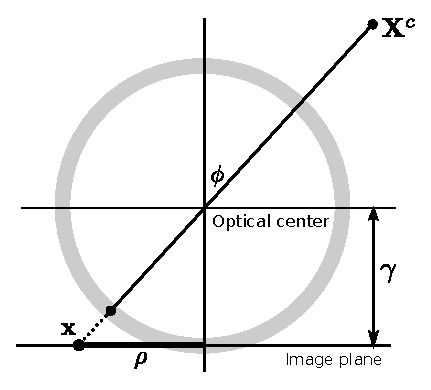
\includegraphics[width=0.48\textwidth]{images/pinholeMapping.eps} &
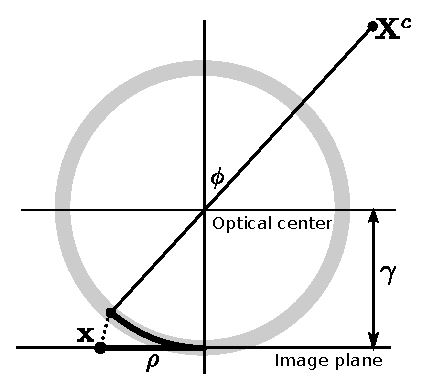
\includegraphics[width=0.48\textwidth]{images/equidistant.eps} \\
(a) & (b) \\
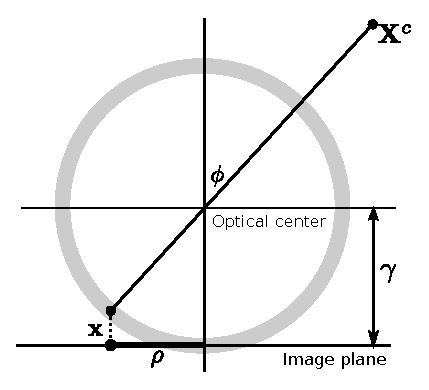
\includegraphics[width=0.48\textwidth]{images/orthographic.eps} &
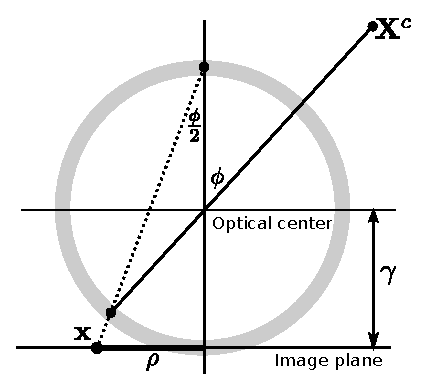
\includegraphics[width=0.48\textwidth]{images/stereographic.eps} \\
(c) & (d)
\end{tabular}
\caption{Illustrations for the mapping functions of the pinhole camera model and the fish-eye camera models. The gray circle denotes a sphere with radius as $\gamma$. (a) The pinhole camera model. (b) The equidistant fish-eye camera model. (c) The orthographic fish-eye camera model. (d) The stereographic fish-eye camera model. }
\label{mappingFig}
\end{figure}


\section{Fish-eye Camera Model}
The field of view of normal cameras is often limited and not wide enough for usage such as robotic navigation. To overcome this drawback, fish-eye cameras with large field of view become prevalent in robotics and computer vision research. In contrary to normal pinhole cameras, fish-eye lens refracts incoming light such that rays from a wide angle can be percepted by a image sensor with limited size. In this section, we briefly introduce the projection property function of fish-eye lens, which is denoted by the mapping function. 

The mapping function is defined about the incident angle $\phi$ of the light with respect to the optical axis. Using the notations from section \ref{pinholeSec}, we denote: 
\begin{equation}
\phi = \text{atan2} (Z^c, \sqrt{{X^c}^2 + {Y^c}^2})
\end{equation}
For simplicity, we assume $\mathbf{d}_\text{rad} = \mathbf{d}_\text{tan} = 0$, $u_0 = v_0 = s = 0$ and $\gamma_1 = \gamma_2 = \gamma$. Thus $\mathbf{m}$ is denoted as
\begin{equation}
\mathbf{m} = \cfrac{\gamma}{Z^c}
\arraycolsep=1.5pt%
\begin{bmatrix}
\begin{array}{c}
X^c \\ Y^c
\end{array}
\end{bmatrix} \\
\end{equation}
This equation can be considered as the mapping function for the pinhole camera model. Denoted by the incident angle $\phi$ we have 
\begin{equation}
\rho = \gamma \tan(\phi)
\label{pinholeMappingEqn}
\end{equation}
where $\rho = \|\mathbf{m}\|$ is the radial coordinate of $\mathbf{m}$. We only consider the radial coordinate $\rho$ here since fish-eye distortion is central radial distortion. An illustration of this mapping function of the pinhole camera model can be found from figure \ref{mappingFig}a. The mapping function of most fish-eye camera models have the similar form with equation \ref{pinholeMappingEqn}. The following are some examples: 
\begin{itemize}
\item \textit{Equidistant}: This is a typical fish-eye model which maintains angular distances. Figure \ref{mappingFig}b shows an illustration of this model. 
\begin{equation}
\rho = \gamma \phi
\end{equation}
\item \textit{Orthographic}: This model is considered to maintain the planar illumination. Figure \ref{mappingFig}c shows an illustration of this model. 
\begin{equation}
\rho = \gamma \sin \phi
\end{equation}
\item \textit{Stereographic}: This is a fish-eye model which maintains angles. Figure \ref{mappingFig}d shows an illustration of this model. 
\begin{equation}
\rho = 2 \gamma \tan(\phi / 2)
\label{stereographicEqn}
\end{equation}
\end{itemize}
More details about the fish-eye camera model can be found from \cite{hughes2010accuracy}. 

\section{Catadioptric Camera Model}
The catadioptric camera model is considered as a unified camera model for different camera model including the pinhole camera and different types of the fish-eye camera model. 
In this toolbox, we consider using the catadioptric camera model as our generic camera model. It is shown in \cite{ying2004can} that the catadioptric model provides a good approximation for modeling fish-eye and wide-angle cameras. A catadioptric camera is an optical system composed by a camera and a curved mirror. The world ``catadioptric'' comes from ``catoptric'' and ``dioptric''. In the catadioptric camra, light is reflected by the curved mirror first and then goes through the camera lens. Figure \ref{cataFig} shows a photo of a catadioptric camera system. Three typically used mirror shape in the catadioptric model is ellipsoid, parabola and hyperbola. 
\paragraph{Parabola Curved Mirror} Figure \ref{cataProjFig}a shows an illustration for the catadioptric camera with a parabola-shaped mirror. An orthogonal camera is assumed to be align with the $xy$ plane. An orthogonal camera is a camera model which transforms a 3D point $[X, Y, Z]^\top$ to $[X, Y]^\top$ on the image plane. It can be interpreted as a pinhole camera with infinite focal length. $xy$ plane is then the image plane of the orthogonal camera. As shown in figure \ref{cataProjFig}a, light which goes through the focal point is reflected to the direction perpendicular to the $x$-axis and then percepted by the orthogonal camera on $xy$ plane. 
\paragraph{Hyperbola Curved and Ellipsoid Curved Mirror} Figure \ref{cataProjFig}b shows an illustration for the catadioptric camera with a hyperbola-shaped mirror. A pinhole camera is located on the lower focal points of the hyperbola. Light which goes through the upper focal point is reflected by the mirror and then percepted by the camera. Thus the camera at the lower focal point can be regarded as a camera on the upper focal point with a much wider field of view. The catadioptric camera with a hyperbola-shaped mirror can be used as an omnidirectional camera as the mirror compresses a wide field of view to a limited range. The ellipsoid mirror is modelled in the similar way but is less used in robotics and computer vision practically. 


\begin{savenotes}
\begin{figure}
\centering
\begin{minipage}{0.457\textwidth}
\centering
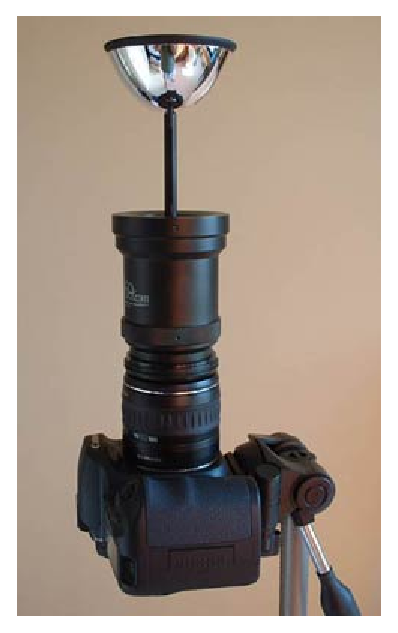
\includegraphics[trim=0in 0in 0in 0in, clip=true, width=1\textwidth]{images/catacamera.eps} \\
(a)
\end{minipage}
\hspace{3pt}
\begin{minipage}{0.512\textwidth}
\centering
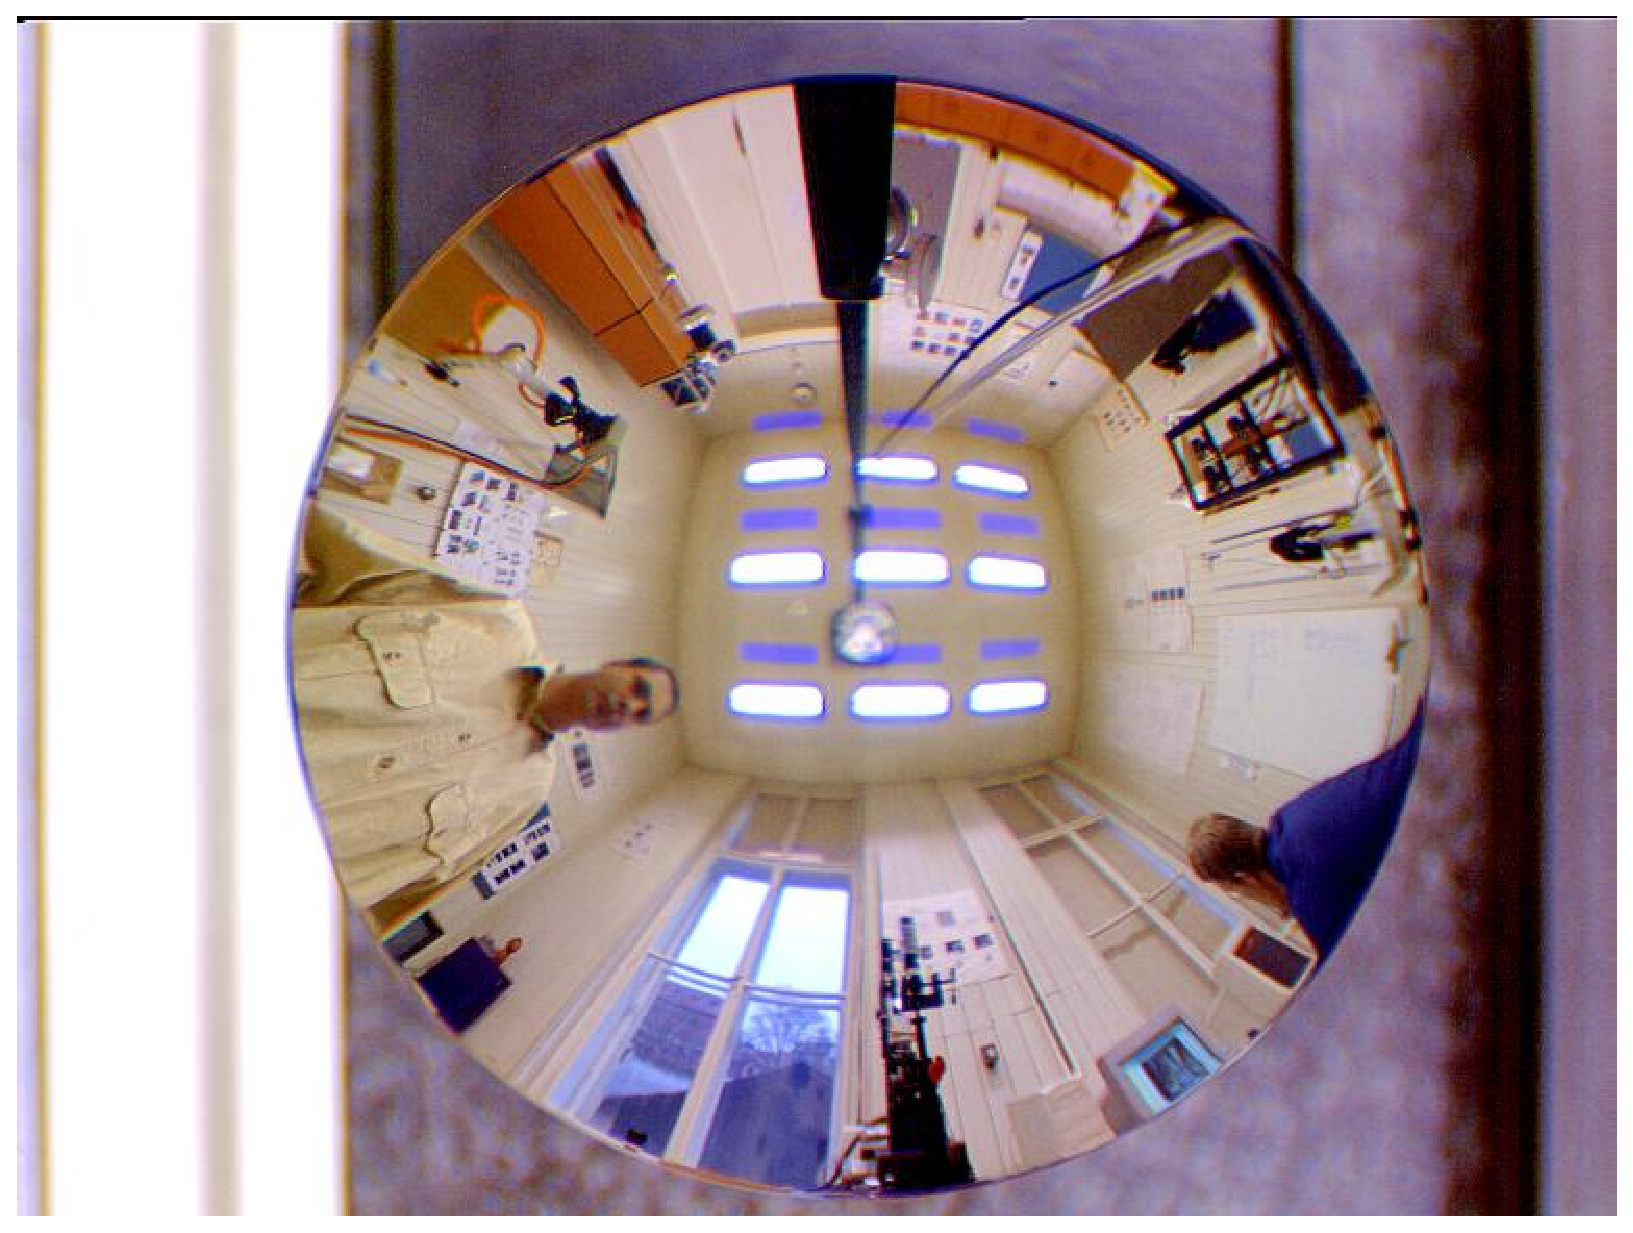
\includegraphics[width=1\textwidth]{images/cataphoto.eps}\\
(b)\\
\includegraphics[width=1\textwidth]{images/undistorted_grobi.eps}\\
(c)
\end{minipage}
\caption{(a) A 0-360 Panoramic Optic \texttrademark \  catadioptric camera system. \protect\footnotemark[1] The system is composed by a curved mirror and a camera. (b) A example image captured by the catadioptric camera with a hyperbola mirror. \protect\footnotemark[2] (c) A example image captured by the fish-eye camera. }
\end{figure}
\end{savenotes}
\footnotetext[1]{Image from \url{http://www.0-360.com}}
\footnotetext[2]{Image from \url{http://cmp.felk.cvut.cz/demos/Omnivis/index.html}}


\begin{figure}
\centering
\begin{tabular}{cc}
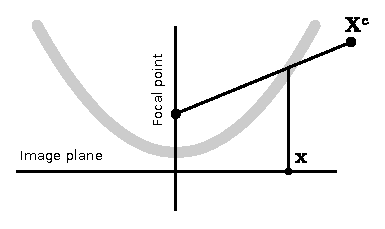
\includegraphics[width=0.48\textwidth]{images/parabola.eps}&
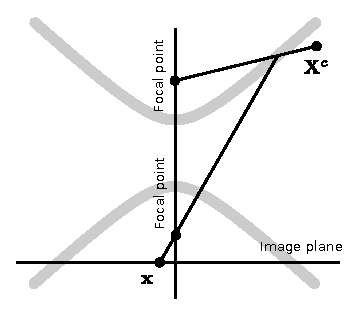
\includegraphics[width=0.48\textwidth]{images/hyperbola.eps}\\
(a) & (b)
\end{tabular}
\caption{Illustrations for the catadioptric camera system. (a) Parabola curved mirror: A parabola curved mirror is plotted as the gray curve. A light ray comes from the 3D point $\mathbf{X}^c$ to the focal point of the parabola. The mirror reflect the ray in the direction which is parallel with the optical axis and perpendicular to the image plane. This configuration forms a orthogonal projection model. The ray is percepted as $\mathbf{x}$ on the image plane. (b) Hyperbola curved mirror: A hyperbola curved mirror is plotted as the gray curve. A light ray comes from the 3D point $\mathbf{X}^c$ to the upper focal point of the hyperbola. The ray is reflected by the mirror to the direction which passes through the lower focal point of the hyperbola. A pinhole camera is located at the lower focal point. The ray is finally percepted as $\mathbf{x}$ on the image plane. }
\label{cataProjFig}
\end{figure}

\bigskip 
The advantage of these three types of the quadratic surface-shaped mirror is that they can be modelled as an equivalent pinhole camera model using the unified projection model proposed by \cite{geyer2000unifying}. Equation \ref{rayEqn} transforms the 3D point $\mathbf{X}^c = [X^c, Y^c, Z^c]^\top$ to its corresponding normalized image point $\mathbf{x} = [x, y]^\top$. In the catadioptric camera model, this transforms is extended by introducing a new parameter $\xi$, which is used to denote the shape of the mirror in the catadioptric model. The ellipsoid-shaped mirror corresponds with $\xi < 1$; The parabola-shaped mirror corresponds with $\xi = 1$; The hyperbola mirror corresponds with $\xi > 1$. The extended transforms is shown as follows: 
\begin{eqnarray}
\mathbf{X}^s &=&
\frac{1}{\| \mathbf{X}^c \|} \mathbf{X}^c \\
x &=& X^s / (Z^s + \xi) \label{liftEqn1}\\
y &=& Y^s / (Z^s + \xi) \label{liftEqn2}
\end{eqnarray}
where $\mathbf{X}^s = [x_s, y_s, z_s]^\top$ is the projection of $\mathbf{X}^c$ on a unit sphere. This transform is shown in figure \ref{cataFig}. Note that the pinhole camera model can also be considered as  special case of the catadioptric camera model with $\xi = 0$. Details about the deduction of the above transform can be found from \cite{geyer2000unifying}. 

Fish-eye, wide-angle and spherical mirror cameras can all be approximately modelled by the catadioptric camera model with some $\xi$. We emphasis here that the stereographic fish-eye camera model can be equivalently denoted by the catadioptric model with $\xi = 1$. Consider equation \ref{stereographicEqn}, we have 
\begin{eqnarray}
\tan(\phi / 2) &=& \rho / (2 \gamma) \\
\tan(\phi) &=& \cfrac{2 \tan(\phi / 2)}{1 - \tan^2(\phi / 2)} = \cfrac{4 \rho \gamma}{4 \gamma^2 - \rho^2}
\end{eqnarray}
Since $\rho = \sqrt{u^2 + v^2}$, the direction of the incident light from $\mathbf{X}^c$ can be denoted as: 
\begin{equation}
\mathbf{X}^c \sim 
\arraycolsep=1.5pt%
\begin{bmatrix}
\begin{array}{c}
4 u \gamma \\ 4 v \gamma \\ 4 \gamma^2 - \rho^2
\end{array}
\end{bmatrix} \sim
\arraycolsep=1.5pt%
\begin{bmatrix}
\begin{array}{c}
u \\ v \\ \cfrac{\gamma'}{2} - \cfrac{1}{2\gamma'} \rho^2
\end{array}
\end{bmatrix} 
\end{equation}
where $\gamma' = \gamma / 2$. As will be shown in section \ref{singleSec}, this formulation is consistent with the catadioptric camera model with $\xi = 1$ and focal length as $\gamma / 2$, that is equation \ref{parabolaEqn}. This fact illustrate the fitness of using the catadioptric model as the unified model for modelling the fish-eye cameras. 


\begin{figure}
\centering
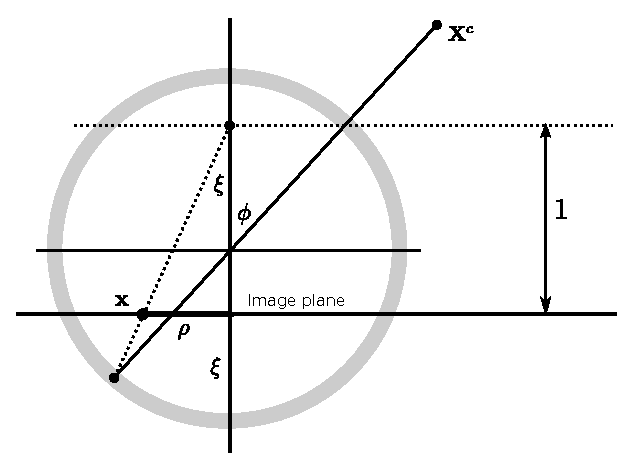
\includegraphics[width = 0.7\textwidth]{images/lift2Dd.eps}
\caption{The unified projection model for the catadioptric camera model. A 3D point $\mathbf{X}^c = [X^c, Y^c, Z^c]^\top$ is firstly projected on a unit sphere and then percepted as $\mathbf{x} = [x, y]^\top$ by an equivalent virtual camera located at $[0, 0, \xi]^\top$. }
\label{cataFig}
\end{figure}

\chapter{Calibration Pattern}
\label{patternSec}
\section{Introduction}
The basic usage of a calibration pattern is to provide easy-to-detect feature points with known 3D coordinates. These features are then detected in the images taken by the camera to be calibrated. The corresponding 2D and 3D points can then be used to estimate the camera parameters. 

Early calibration research, for example the Direct Linear Transform (DLT) method \cite{abdelaziz1971} (see section \ref{singleSec} for more details), uses perpendicular jointed planes as the calibration object. A coordinate system can be easily defined to be aligned with the gridded plane. Coordinates of the square corners or the dots can then be measured in this coordinate system. Figure \ref{calibPattFig}a shows an example of the calibration object. Define the intersection line of the two chessboards as the $z$ axis and the bottom line of the two chessboards as $x$ and $y$ axes respectively. The 3D coordinates of each chessboard corner are then defined. The usage of this type of calibration object is limited by two drawbacks: 1) It is not flexible and convenient to move large jointed planes if the camera is fixed somewhere such as on a car or on a wall; 2) It is difficult to joint the two planes perfectly orthogonal. 

\begin{savenotes}
\setlength{\tabcolsep}{2pt}
\begin{figure}
\centering
\begin{tabular}{ccc}
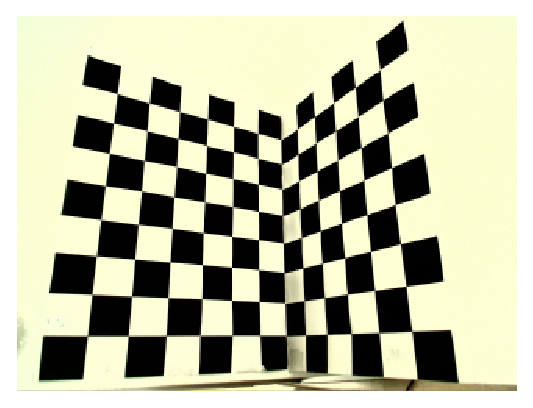
\includegraphics[width=0.33\textwidth]{images/calibpatt/calib-cube.eps} &
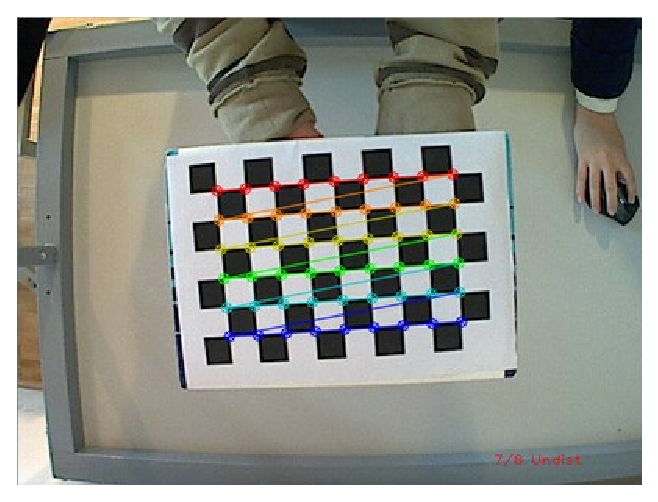
\includegraphics[width=0.33\textwidth]{images/calibpatt/calib-chessboard.eps} & 
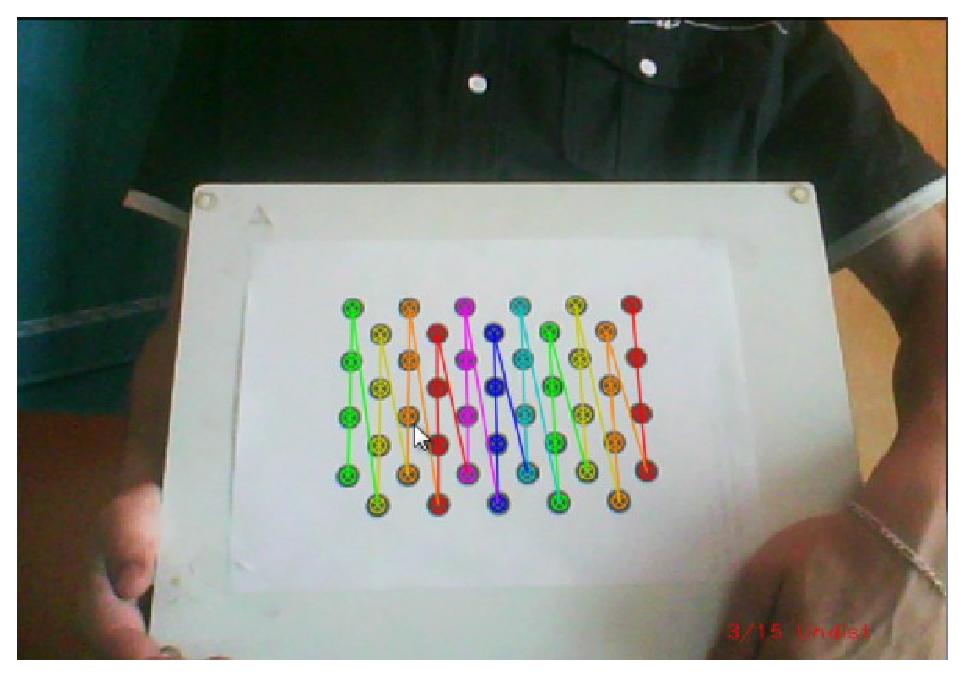
\includegraphics[trim=0.3in 0in 0.2in 0in, clip=true, width=0.33\textwidth]{images/calibpatt/calib-dot.eps} \\
(a) & (b) & (c)\\
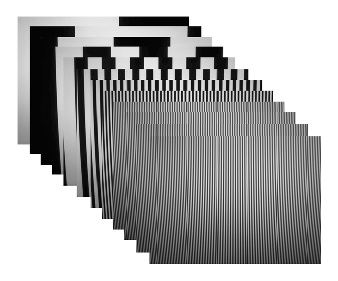
\includegraphics[width=0.33\textwidth]{images/calibpatt/calib-temporal.eps} &
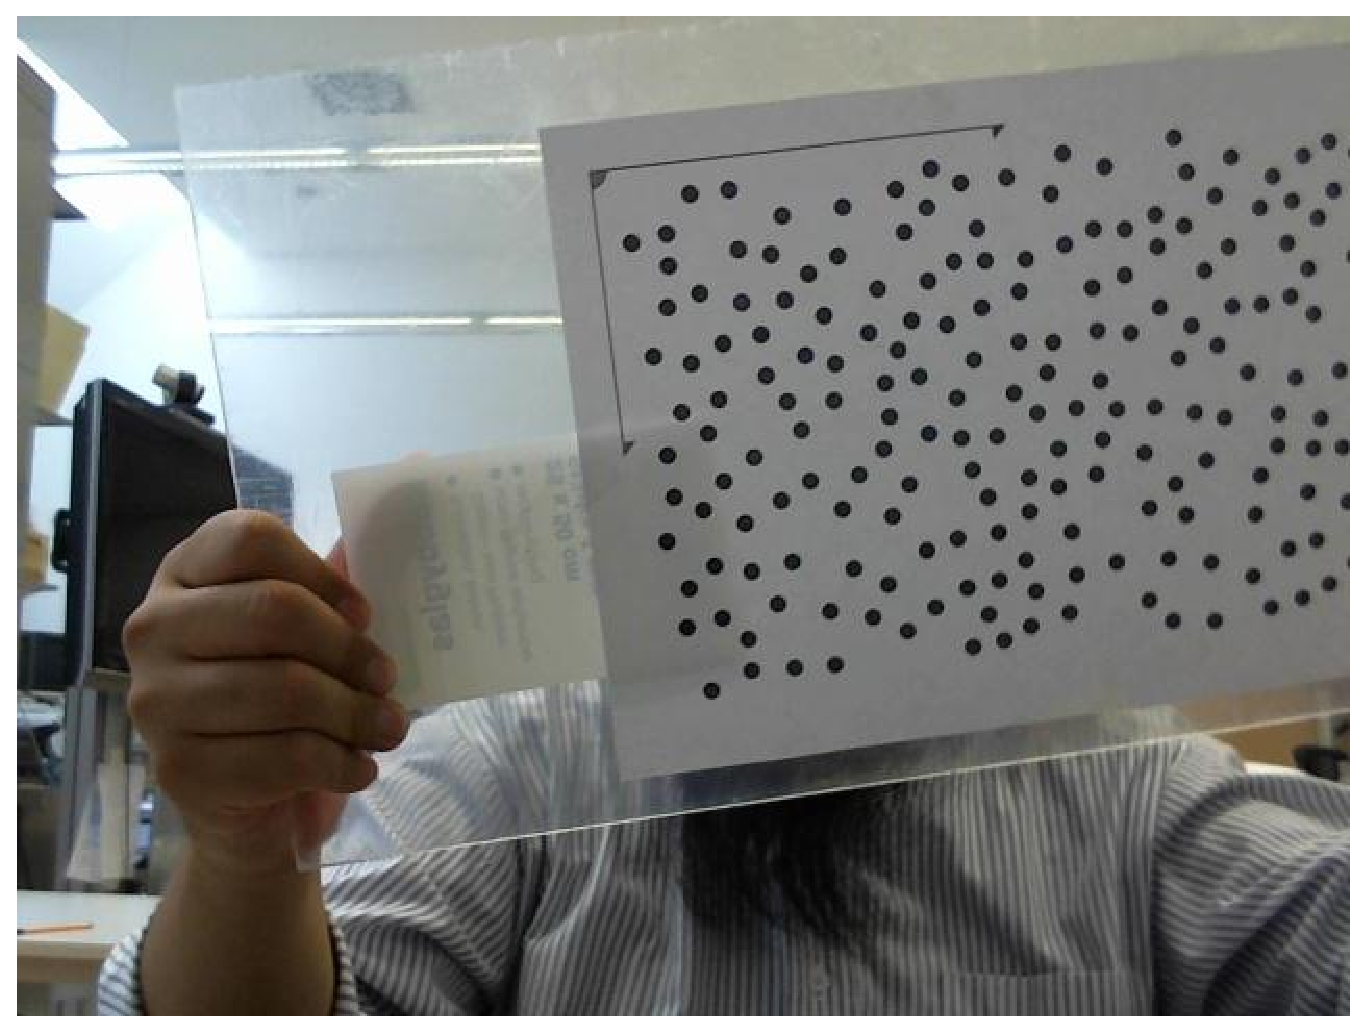
\includegraphics[width=0.33\textwidth]{images/calibpatt/calib-randot.eps} & 
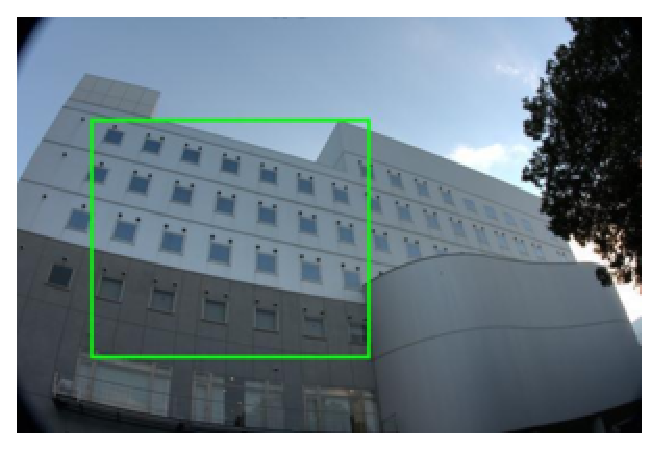
\includegraphics[trim=0.3in 0in 0.2in 0in, clip=true, width=0.33\textwidth]{images/calibpatt/calib-rank.eps} \\
(d) & (e) & (f)
\end{tabular}
\caption{(a) An example of the calibration object made up of two perpendicular chessboard plane.\protect\footnotemark[1] (b) An example of the chessboard pattern. The colored line marks the automatically detected chessboard corners. \protect\footnotemark[2] (c) An example of the dot pattern. The colored line marks the automatically detected dots. \protect\footnotemark[3] (d) An example image sequence of the temporal coded calibration pattern. \protect\footnotemark[4] (e) An example image of the random dots calibration pattern. \protect\footnotemark[5] (f) An example image of the low-rank calibration pattern. \protect\footnotemark[6]}
\label{calibPattFig}
\end{figure}
\end{savenotes}
\footnotetext[1]{Image from \url{http://cvg.ethz.ch/teaching/2012fall/compvis/}. }
\footnotetext[2]{Image from \cite{opencv_library}. }
\footnotetext[3]{Image from \cite{opencv_library}. }
\footnotetext[4]{Image from \cite{schmalz2011camera}. }
\footnotetext[5]{Image from \cite{oyamadasingle}. }
\footnotetext[6]{Image from \cite{zhang2011camera}. }
As later research \cite{tsai1987versatile, zhang2000flexible} proposes more convenient calibration method using 3D points from only one plane, plane calibration objects become most widely used in recent research on camera calibration. A variety of 2D calibration patterns are proposed. Here we provide an overview of some existing 2D calibration pattern. This overview compares the patterns in the following two aspects: 1) The accuracy of feature detection; 2) The difficulty of automatic feature detection and matching. 


\paragraph{Chessboards and gridded dots} Figures \ref{calibPattFig}b and \ref{calibPattFig}c show images of the two patterns. These patterns are the most widely used calibration pattern in current camera calibration research. Discussion about the accuracy of these two pattern can be found from \cite{mallon2007pattern}. The chessboard corner detection is well-known to be sub-pixel accurate and unbiased, while the dot detection maybe biased due to the distortion of the cameras. Automatic detection for this two pattern is both possible and many available detection packages can be obtained online \cite{opencv_library, rufli2008automatic, geiger2012automatic}. 
	The drawback of these two patterns is that the detected corners or dots are ambiguous and do not have descriptors. To match the detected image points with the corresponding pattern points, current automatic pattern detector search for the entire grid structure. This method requires that the entire grid of the chessboard or the dots be visible. Thus the detector can not handle the cases when the pattern is partly occluded. As mentioned in section \ref{motiveSec}, this limit makes the chessboard and dot pattern not suitable for calibrating many multiple-camera systems whose cameras have little overlapping field of view. In addition, the detection might fail when the feature density is very high, since in this case it is difficult to detect all features on the pattern. 
%	\item \textit{Pattern with spatial coded features} The ambiguity of the features on the calibration pattern can be solved by assigning each feature a code. Figure \ref{} shows an example of a spatial code compose by 2D ?bar code?. Some research about the code design can be found from \cite{}. Using coded features, detected image features can be matched to their corresponding pattern features easily by matching the codes. Thus the pattern is not required to be entirely visible in the image. The drawback of the 2D ?bar code? is that the bar detection assumes a perspective camera model, which is not suitable when calibrating a camera with high distortion. In addition, the features on the pattern can not be dense as the ?bar codes? have to be large enough and well separated to be detected. 
\paragraph{Pattern with time-coded features} \cite{scharstein2003high} proposes a well-known method to use time-coded features to generate stereo vision benchmark. The same idea can be applied for camera calibration. In \cite{grosse2012camera, schmalz2011camera}, a display screen is used to display the calibration pattern. The brightness of each point on the display is changing according to a unique code. For each camera pose, a sequence of images are taken to percept the entire temporal code. Then the points are indexed and matched by the code. The advantage of the time-coded pattern is that the feature density can be very high and that the correspondence matching is not affected by occlusion. However, using the time-coded pattern in calibration is not very convenient. It requires a monitor or a projector to display the pattern, a tripod to fix the camera and many more images to be taken to percept the code. Figure \ref{calibPattFig}d shows an example for the temporal coded calibration pattern. 
\paragraph{Random dots pattern} \cite{oyamadasingle} shows that if dots are randomly distributed on the calibration pattern, the local dots distribution can be used to identify the feature correspondence. Figure \ref{calibPattFig}d shows an example of this random dot pattern. Some geometric invariance is computed as a descriptor for each dot from the local nearest dot set. The drawback of this method is the poor robustness under significant camera distortion. 
\paragraph{Low rank pattern} \cite{zhang2011camera} proposes a novel calibration method which does not require any specific calibration pattern. The method can calibrate a camera using any pattern with low rank texture. For example, periodic rectangular structures such as chessboards and building facets can all be used. The method searches for an optimal camera parameters so that the rank of the reprojected pattern is minimized. This method is convenient for scenarios where no calibration object is available. The drawback is that the calibration accuracy is affected by the quality of the selected pattern and that manual selection for the pattern area is required. 


In this paper, we seek to design a new calibration pattern to improve the drawbacks of the above patterns. The new pattern is required to have the following properties: 1) The feature can be detected accurately on an image; 2) The feature can be automatically detected easily; 3) The feature point is coupled with a distinguishable descriptor so that correspondences can be matched easily even with occlusion; 3) The pattern consists of sufficient features; 4) The pattern should be easy to be displayed or printed on a normal board. A pattern with such properties is very useful for calibrating multiple-camera system with minimal overlapping field of view. In the following sections in this chapter, we shows that a pattern which consists of suffient SIFT or SURF features \cite{lowe2004distinctive, bay2006surf} is a good design fulfilling the above requirements. 


\begin{figure}
\centering
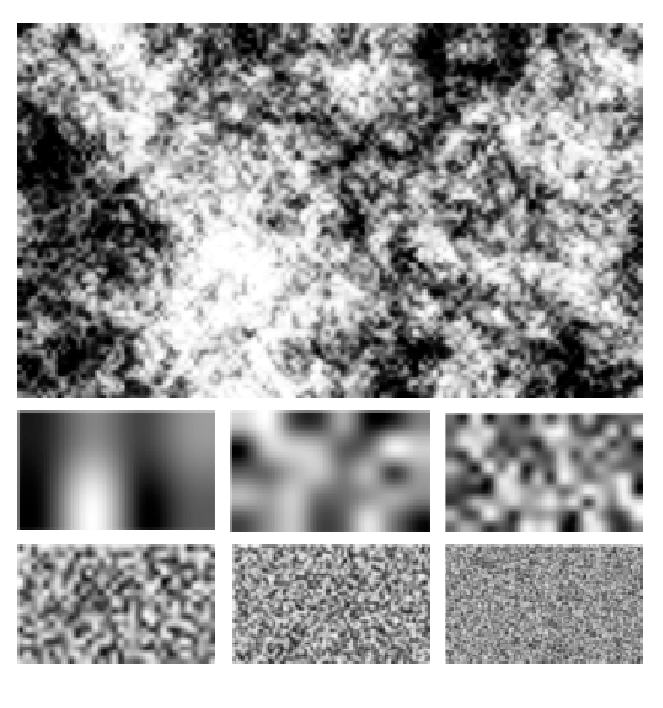
\includegraphics[width=0.6\textwidth]{images/patternsample}
\caption{Top: The proposed calibration pattern. Bottom: Image components with noise at different frequencies.}
\label{PatternFig}
\end{figure}


\label{PatternSec}
\section{Feature Detection Revisited}
%TODO Added sift feature figures and more details. 

Point-feature detection is a computer vision technique widely and successfully applied to many areas such as sparse reconstruction and object detection. A point feature typically contains two components: a keypoint and a descriptor. We look at the widely-used SIFT implementation \cite{lowe2004distinctive} as a example. A Difference of Gaussian filter (DoG) is used to detect key points. This detection is executed on both the original image and downsampled images; in short, keypoint detection is done on different scales. For each keypoint, the image gradient in the keypoint's neighborhood is converted to a histogram which is then used as the descriptor for the corresponding feature point. SURF, a variant of SIFT, is also a widely-used feature detection and descriptor extraction technique \cite{bay2006surf}. SURF replaces SIFT in many applications due to the its computational efficiency. In the proposed toolbox, we use SURF features. 

\section{Reverse Engineering}
The basic idea behind the proposed calibration pattern is to design a pattern which consists of sufficient detectable features. At the same time, the feature descriptors should be highly discriminative so that we can easily obtain unique feature point matches. 

To facilitate feature detection, we use several noise images to compose a calibration pattern in accordance with the mechanism of SIFT/SURF. The DoG filter applied to a noise image can yield points with high response. However, a problem with high-frequency image noise is the blurring effect. For a grayscale image, if the camera is located far away, the noise image is perceived as a purely gray image. The solution to this problem is to compose images with noise from multiple scales. In our implementation, we generate noise images of different sizes, and resize them such that they have the same size. These images with noise on different scales are then added up together. This procedure can be interpreted as a reverse engineering of the scaling procedure in SIFT/SURF detection. Thus, the resulting image contains a high number of detectable features on different scales; such features can be detected by a camera at varying distances. The Matlab in figure \ref{patternCodeFig} generates a $600 \times 800$ calibration pattern. Figure \ref{PatternFig} shows a calibration pattern at the top, and its components with noise on different scales at the bottom. 

\small
\begin{verbbox}
N = 600; M = 800;
pattern = 0; count = 0;
m = 4;
while m < M
  n = round(N / M * m);
  noise = rand(n, m);
  noise = imresize(noise, [N, M]);
  pattern = pattern + noise;
  count = count + 1;
  m = m * 2;
end
pattern = pattern ./ count;
pattern = histeq(pattern);
imshow(pattern);
\end{verbbox}
\normalsize

\begin{figure}
  \centering
  \theverbbox
  \caption{Matlab code for pattern generation.}
  \label{patternCodeFig}  
\end{figure}


\section{Feature Matching}
Feature detection and feature matching between images are two standard steps of in a modern 3D vision pipeline. In our calibration approach, we employ a similar step to match features between each image and the known calibration pattern image. First, features detected from each image and the pattern image are matched according to the descriptor similarity. We use the well-known distance ratio check proposed in \cite{lowe2004distinctive}. For a set of at least 2 candidate matches for each query feature, the best match is accepted only if its descriptor distance is smaller than 0.6 times the descriptor distance between the query feature and its second best match. 

Next, a \textit{fundamental matrix for radial distortion} is estimated by RANSAC between the image points and pattern points to find inlier point correspondences. Note that this fundamental matrix is analogous to but not the same with the fundamental matrix used in traditional epipolar geometry. The traditional matrix requires that point correspondences have image coordinates corresponding to rectified images. Details about this fundamental matrix can be found in \cite{hartley2007parameter}. We provide some simple explanation about the fundamental matrix for radial distortion here. The fundamental matrix for radial distortion assumes that only radial lens distortion. 

Consider the distorted and undistorted image point, $\mathbf{x}'$ and $\mathbf{x}$ on the normalized image plane. Denote their homogeneous coordinates as $\mathbf{p}'$ and $\mathbf{p}$, respectively. If the image only has radial distortion and $\mathbf{e}$ is the distortion center, we can write:
\begin{equation}
\mathbf{p}' = \mathbf{e} + \lambda (\mathbf{p} - \mathbf{e})
\end{equation}
where $\lambda$ is a distortion coefficient corresponding to $\mathbf{x}$. Consider its corresponding 3D point $\mathbf{X}^w = [X^w, Y^w, 0]^\top$ on the calibration pattern, which is aligned with the plane $z = 0$. From equations \ref{cmEqn1} and \ref{rayEqn}, we have
\begin{equation}
\begin{split}
\mathbf{p} \sim 
\arraycolsep=1.5pt%
\begin{bmatrix}
	\begin{array}{c}
	X^c \\ Y^c \\ Z^c
	\end{array}
\end{bmatrix} 
= 
\begin{bmatrix}
\mathbf{R} & \mathbf{t}
\end{bmatrix}
\arraycolsep=1.5pt%
\begin{bmatrix}
	\begin{array}{c}
	\mathbf{X}^w \\ 1
	\end{array}
\end{bmatrix}
= 
\begin{bmatrix}
\mathbf{r}_1 & \mathbf{r}_2 & \mathbf{r}_3 & \mathbf{t}
\end{bmatrix}
\arraycolsep=1.5pt%
\begin{bmatrix}
	\begin{array}{c}
	X^w \\ Y^w \\ 0 \\ 1
	\end{array}
\end{bmatrix}\\
= 
\begin{bmatrix}
\mathbf{r}_1 & \mathbf{r}_2 & \mathbf{t}
\end{bmatrix}
\arraycolsep=1.5pt%
\begin{bmatrix}
	\begin{array}{c}
	X^w \\ Y^w \\ 1
	\end{array}
\end{bmatrix}
=\mathbf{H}
\arraycolsep=1.5pt%
\begin{bmatrix}
	\begin{array}{c}
	X^w \\ Y^w \\ 1
	\end{array}
\end{bmatrix}
\end{split}
\end{equation}
$\mathbf{H}$ is a homography from the calibration pattern plane $z = 0$ to the normalized image plane. Denote $\mathbf{p}^w = [X^w, Y^w, 1]^\top$. We assume that $\mathbf{H}$ is multiplied by a proper scale factor such that: 
\begin{equation}
\mathbf{p} = \mathbf{H} \mathbf{p}^w
\end{equation}
Substituting this into the above equation, we obtain: 
\begin{equation}
\mathbf{p}' = \mathbf{e} + \lambda (\mathbf{H} \mathbf{p}^w - \mathbf{e})
\end{equation}
Consider the cross product between the equation and $\mathbf{e}$, we get:
\begin{equation}
{}\mathbf{e} \times \mathbf{p}' = \lambda (\mathbf{e} \times \mathbf{H}) \mathbf{p}^w
\end{equation}
Left-multiplying the equation again by ${\mathbf{p}'}^\top$, we get:
\begin{equation}
0 = {\mathbf{p}'}^\top (\mathbf{e} \times \mathbf{H}) \mathbf{p}^w
\end{equation}
Note that $\mathbf{p}'$ is on the normalized image plane. We relate $\mathbf{p}'$ with $\mathbf{m}$ by equation \ref{cmEqn4} as: 
\begin{equation}
\arraycolsep=1.5pt%
\begin{bmatrix}
	\begin{array}{c}
	\mathbf{m}\\ 1
	\end{array}
\end{bmatrix} = 
\mathbf{K}
\mathbf{p}'
\end{equation}
Thus we have 
\begin{equation}
0 = 
\begin{bmatrix}
	\mathbf{m}^\top & 1
\end{bmatrix} 
\mathbf{K}^{-1} (\mathbf{e} \times \mathbf{H}) \mathbf{p}^w
\end{equation}
$\mathbf{F} \equiv \mathbf{K}^{-1} (\mathbf{e} \times \mathbf{H})$ is the fundamental matrix for radial distortion, and $\mathbf{e}$ can be regarded as the principal point. This fundamental matrix is well-suited to both the pinhole and unified projection models, and is used to remove false feature matches in our proposed calibration approach. $\mathbf{p}^w$ denotes the point detected from the original pattern and $[\mathbf{m}, 1]^\top$ denotes the point detected from the image. Only in case the images perfectly agree with the pinhole camera model (no lens distortion at all), the fundamental matrix degenerates and can not be estimated uniquely. This case suffices to estimate a homography from the 3D world point to the normalized image point. 
This case could be detected by automatic model selection methods like the GRIC criterion \cite{torr1997assessment}, however since this is a very special case, for the current version we leave it to the user to specify this mode.
% However, this fundamental matrix for radial distortion is degenerate when the features are perfectly undistorted. In this case, a homography can be estimated between the pattern features and image features. We select the correct model by comparing the number of inliers.  investigates more complex model selection methods; however, we do not use such methods in our toolbox for sake of simplicity. 

\chapter{Single-Camera Calibration}
\label{singleSec}

\section{Introduction}
The single-camera calibration estimates the camera intrinsics and the poses of the calibration pattern with respect to the camera's coordinate system. Methods for calibrating a single camera have been well studied in the past decades. The calibrated camera intrinsics and pattern poses for each single cameras can then be used in calibrating the multiple-camera system formed by these single cameras. In this chapter, we firstly provide a brief introduction to some of the state-of-art single camera calibration methods and secondly illustrate the single camera calibration method used in our proposed toolbox. 



\subsection{Related Work}
Most commonly used camera calibration methods can be formed as a two-stage procedure. The first stage is the initialization of camera parameters and the second stage is the refinement of the parameters. In this subsection we provide an introduction of the state-of-art single camera calibration approaches, mainly focusing on the initialization stage, since the refinement stage is roughly similar for different calibration approaches. 

\subsubsection{Direct Linear Transform (DLT) Method for Pinhole Camera Calibration}
First we introduce the basic idea of the well-known DLT calibration method proposed by \cite{abdelaziz1971}. Since the distortion coefficients are usually small, we assume that the distortion coefficients $k_1 = k_2 = p_1 = p_2 = 0$ at the initialization stage. Combining equations \ref{cmEqn1}--\ref{cmEqn4}, we obtain the following equations for the pinhole camera projection model, with zero lens distortion. 
\begin{eqnarray}
\mu \arraycolsep=1.5pt%
\begin{bmatrix}
	\begin{array}{c}
	\mathbf{m} \\ 1
	\end{array}
\end{bmatrix}
 &=& \mathbf{P} 
\arraycolsep=1.5pt%
\begin{bmatrix}
	\begin{array}{c}
	\mathbf{X}^w \\ 1
	\end{array}
\end{bmatrix} \\
\mathbf{P} &=& \mathbf{K} 
\begin{bmatrix}
\mathbf{R} & \mathbf{t}
\end{bmatrix} 
\end{eqnarray}
where $\mu$ is a scale factor. Given a set of known 3D points $\mathbf{X}^w_i = [X_i^w, Y_i^w, Z_i^w]^\top$ and their corresponding image points $\mathbf{m}_i = [u_i, v_i]$ from a single image. $\mathbf{P}$ can be solved from the following equation system 
\begin{equation}
\arraycolsep=1.5pt%
\begin{bmatrix}
	\begin{array}{c}
	\mathbf{m}_i \\ 1
	\end{array}
\end{bmatrix}
 \times \mathbf{P} 
\arraycolsep=1.5pt%
\begin{bmatrix}
	\begin{array}{c}
	\mathbf{X}^w_i \\ 1
	\end{array}
\end{bmatrix}
 = 0, i = 1, 2, 3, \dots
\label{dltLS}
\end{equation}
The first 3 columns of $\mathbf{P}$ is equal to $\mathbf{K} \mathbf{R}$, where $\mathbf{R}$ is the rotation matrix of the pattern when it is captured in the single image. From equation \ref{kEqn}, we know $\mathbf{K}$ is a upper-triangular matrix. Thus, $\mathbf{K}$ and $\mathbf{R}$ can be obtained by executing an RQ-decomposition (a variation of the well-known QR decomposition) on the first 3 columns of $\mathbf{P}$ and $\mathbf{t}$ can be extracted from $\mathbf{P}$. In addition, some techniques of linearly solving the radial lens distortion can be found in \cite{abdelaziz1971}. 

After we obtain these initial estimation for the camera parameters, a non-linear refinement can be executed to obtain the final estimation of the camera parameters. The refinement starts from the initial estimated $\mathbf{K}$, $\mathbf{R}$, $\mathbf{t}$ and zero distortion. It varies these parameters to minimize summarized reprojection error of all the 3D points $\mathbf{X}^w$. The minimization problem is formed as follows: 
\begin{equation}
\begin{aligned}
& \argmin_{\mathbf{R}, \mathbf{t}, \mathcal{C}} & & \sum_{\forall i} \left \| \mathbf{m}_i - \hat{\mathbf{m}}_i(\mathbf{X}^w_i, \mathbf{R}, \mathbf{t}, \mathcal{C}) \right \|^2
\end{aligned}
\label{dltOptEqn}
\end{equation}
where $\hat{\mathbf{m}}_i(\star)$ denotes the camera projection procedure formed by equations \ref{cmEqn1}-\ref{cmEqn4}. $\mathcal{C}$ denotes all the intrinsic parameters of the camera. If multiple images of a calibration object is available, we can initialize the calibration using one image and then minimize the reprojection error of all the images. Thus the summarized reprojection error is formed as: 
\begin{equation}
\begin{aligned}
& \argmin_{\mathbf{R}_i, \mathbf{t}_i, \mathcal{C}, \forall i} & & \sum_{\forall i, \forall j} \left \| \mathbf{m}_{i, j} - \hat{\mathbf{m}}_{i, j}(\mathbf{X}^w_{i, j}, \mathbf{R}_i, \mathbf{t}_i, \mathcal{C}) \right \|^2
\end{aligned}
\label{dltAllOptEqn}
\end{equation}
Here $i$ is used to index different images and $j$ is used to index different points. The DLT method requires calibration objects such as two perpendicular calibration patterns shown in figure \ref{calibPattFig}a. If 3D points are only located on same plane, as is the case for all the planar calibration objects, the DLT method will degenerate and there is no unique solution. We provide a simple illustration for this degeneration. If 3D points are all on a plane, we can denote these points as $\mathbf{X}^w = [X^w, Y^w, 0]^\top$. In equation \ref{dltLS}, the third column of $\mathbf{P}$ is always multiplied by 0 and can not be solved. 

\subsubsection{Zhang's Method for Pinhole Camera Calibration}
The current most widely used calibration method for the pinhole camera model is the method proposed by \cite{zhang2000flexible}. We introduce the basic idea for this method at the initialization stage with zero lens distortion $k_1 = k_2 = p_1 = p_2 = 0$ assumed. This method only requires a plane as the calibration object. Define the $xy$ plane of world coordinate system to be aligned with the calibration pattern, for example the chessboard grids. Then the 3D world point, which is the chessboard corner, can be denoted as $\mathbf{X}^w = [X^w, Y^w, 0]^\top$. Denote $\mathbf{R} = [\mathbf{r}_1, \mathbf{r}_2, \mathbf{r}_3]$, we can write the camera transform as: 
\begin{equation}
\begin{split}
\mu \arraycolsep=1.5pt%
\begin{bmatrix}
	\begin{array}{c}
	\mathbf{m} \\ 1
	\end{array}
\end{bmatrix} = \mathbf{K}
\begin{bmatrix}
\mathbf{R} & \mathbf{t}
\end{bmatrix}
\arraycolsep=1.5pt%
\begin{bmatrix}
	\begin{array}{c}
	\mathbf{X}^w \\ 1
	\end{array}
\end{bmatrix}
= \mathbf{K}
\begin{bmatrix}
\mathbf{r}_1 & \mathbf{r}_2 & \mathbf{r}_3 & \mathbf{t}
\end{bmatrix}
\arraycolsep=1.5pt%
\begin{bmatrix}
	\begin{array}{c}
	X^w \\ Y^w \\ 0 \\ 1
	\end{array}
\end{bmatrix}\\
= \mathbf{K}
\begin{bmatrix}
\mathbf{r}_1 & \mathbf{r}_2 & \mathbf{t}
\end{bmatrix}
\arraycolsep=1.5pt%
\begin{bmatrix}
	\begin{array}{c}
	X^w \\ Y^w \\ 1
	\end{array}
\end{bmatrix}
=\mathbf{H}
\arraycolsep=1.5pt%
\begin{bmatrix}
	\begin{array}{c}
	X^w \\ Y^w \\ 1
	\end{array}
\end{bmatrix}
\end{split}
\end{equation}
where $\mathbf{H} = [\mathbf{h}_1, \mathbf{h}_2, \mathbf{h}_3]$ is a homography from the calibration pattern plane to the image plane. By stacking a set of point correspondences between the calibration pattern and the image, $\mathbf{H}$ can be solved up to an unknown scale. Given that $\mathbf{r}_1$ and $\mathbf{r}_2$ is two columns of a rotation matrix. We have the following constraints: 
\begin{eqnarray}
\mathbf{h}_1^\top \mathbf{K}^{-\top} \mathbf{K}^{-1} \mathbf{h}_2 &=& 0 \\
\mathbf{h}_1^\top \mathbf{K}^{-\top} \mathbf{K}^{-1} \mathbf{h}_1 &=& \mathbf{h}_2^\top \mathbf{K}^{-\top} \mathbf{K}^{-1} \mathbf{h}_2
\end{eqnarray}
where $\mathbf{r}_1 \sim \mathbf{K}^{-1} \mathbf{h}_1$ and $\mathbf{r}_2 \sim \mathbf{K}^{-1} \mathbf{h}_2$, both with a same unknown scale. The above are two linear constraints on matrix $\mathbf{K}^{-\top} \mathbf{K}^{-1}$. If we have $N \geq 3$ images taken at different positions, $\mathbf{K}^{-\top} \mathbf{K}^{-1}$ can be uniquely solved by forming a linear system using $\mathbf{H}$ from different images. And then $\mathbf{K}$ can be extracted by matrix decomposition. 

In addition, some techniques of linearly solving the radial lens distortion can be found in \cite{zhang2000flexible}. After the initial calibration estimation is obtained, a refinement can be executed similarly to equation \ref{dltAllOptEqn}. 

The calibration toolboxes by Bouguet \cite{bouguet2004camera} and OpenCV \cite{opencv_library} implement Zhang's calibration method. These toolboxes are currently the most widely used camera calibration toolboxes for pinhole camera model. 

\subsubsection{Mei's Method for Catadioptric Camera Calibration}
\cite{mei2007single} proposes a method for easily calibrating the catadioptric camera. The method firstly assumes $\xi = 1$, $k_1 = k_2 = p_1 = p_2 = 0$, $\gamma_1 = \gamma_2 = \gamma$ and the principal point $[u_0, v_0]^\top$ to be at the center of the image. For an image point $\mathbf{m} = [u, v]^\top$, its corresponding normalized image point $\mathbf{x} = [x, y]^\top$ can be obtained as:
\begin{eqnarray}
x = (u - u_0) / \gamma \\
y = (v - v_0) / \gamma
\end{eqnarray}
Substitute $\mathbf{x} = [x, y]^\top$ to equations \ref{liftEqn1} and \ref{liftEqn2}, we obtain the ray which goes from the camera center to $\mathbf{X}^c$ as: 
\begin{equation}
\mathbf{X}^c \sim \mathbf{X}^s \sim
\arraycolsep=1.5pt%
\begin{bmatrix}
	\begin{array}{c}
	u - u_0 \\ v - v_0 \\ \cfrac{\gamma}{2} - \cfrac{1}{2 \gamma} \rho^2
	\end{array}
\end{bmatrix} 
\label{meiRayEqn}
\end{equation}
where $\rho = \sqrt{(u - u_0)^2 + (v - v_0)^2}$. Details about the deduction can be found from \cite{mei2007single}. For an image point $\mathbf{m}$, its corresponding 3D ray is obtained as the above vector. In \cite{mei2007single}, the author selects a set of point located on a line on the chessboard and stacks their corresponding rays in a matrix as:
\begin{equation}
\arraycolsep=1.5pt%
\begin{bmatrix}
	\begin{array}{ccc}
	u_1 - u_0\  & v_1 - v_0\  & \cfrac{\gamma}{2} - \cfrac{1}{2 \gamma} \rho_1^2 \\
	u_2 - u_0\  & v_2 - v_0\  & \cfrac{\gamma}{2} - \cfrac{1}{2 \gamma} \rho_2^2 \\
	&\cdots	&
	\end{array}
\end{bmatrix} 
\end{equation}  
Since the selected points are on a line in the 3D space, their corresponding rays are on a same plane. Thus the above matrix should have a rank of 2. By enforcing this rank constraints, $\gamma$ can be solved. The extrinsics $\mathbf{R}$ and $\mathbf{t}$ for each image can be initialized using the PnP algorithm \cite{gao2003complete}. 

After we obtain the initial values of both intrinsic parameters and the camera pose with respect to the chessboard, an overall refinement can be executed to compute the final calibration result similarly to equation \ref{dltAllOptEqn}. 

Mei's method is a very easy-to-use calibration technique for catadioptric camera model. \cite{mei2007single} also shows that it can also be used to calibrate wide-angle and fisheye camera accurately. The only drawback is that it requires points on a line on the calibration pattern to initialize the focal length. This is not applicable for our proposed pattern with random noise, where no line structure is available. In our proposed approach, we resolve this drawback by selecting a different initialization technique. 

\subsubsection{Scaramuzza's Method for Generic Camera Calibration}
Scaramuzza \cite{scaramuzza2006toolbox} proposes a more general model than Mei's methd. The calibration method in \cite{scaramuzza2006toolbox} does not assume any specific projection model for the camera. In analogy to equation \ref{meiRayEqn}, \cite{scaramuzza2006toolbox} parametrize a 3D ray corresponding to a image point $\mathbf{m}$ using polynomial approximation as: 
\begin{equation}
\mathbf{X}^c \sim \mathbf{X}^s \sim
\arraycolsep=1.5pt%
\begin{bmatrix}
	\begin{array}{c}
	u - u_0 \\ v - v_0 \\ a_0 + a_1 \rho + \cdots + a_n \rho^n
	\end{array}
\end{bmatrix} 
\label{scaraRayEqn}
\end{equation}
where $\rho = \sqrt{(u - u_0)^2 + (v - v_0)^2}$ and $a_0, \cdots, a_n$ are a set of distortion parameters to be estimated. The calibration method uses planar calibration pattern and is initialized via the following steps. 
\begin{equation}
\mathbf{X}^c = 
\begin{bmatrix}
\mathbf{R} & \mathbf{t}
\end{bmatrix}
\arraycolsep=1.5pt%
\begin{bmatrix}
	\begin{array}{c}
	\mathbf{X}^w \\ 1
	\end{array}
\end{bmatrix}
= 
\begin{bmatrix}
\mathbf{r}_1 & \mathbf{r}_2 & \mathbf{r}_3 & \mathbf{t}
\end{bmatrix}
\arraycolsep=1.5pt%
\begin{bmatrix}
	\begin{array}{c}
	X^w \\ Y^w \\ 0 \\ 1
	\end{array}
\end{bmatrix}
= 
\begin{bmatrix}
\mathbf{r}_1 & \mathbf{r}_2 & \mathbf{t}
\end{bmatrix}
\arraycolsep=1.5pt%
\begin{bmatrix}
	\begin{array}{c}
	X^w \\ Y^w \\ 1
	\end{array}
\end{bmatrix}
\label{planarEqn}
\end{equation}
Combining with equation \ref{scaraRayEqn}, we have: 
\begin{equation}
\arraycolsep=1.5pt%
\begin{bmatrix}
	\begin{array}{c}
	u - u_0 \\ v - v_0 \\ a_0 + a_1 \rho + \cdots + a_n \rho^n
	\end{array}
\end{bmatrix} 
\times
\begin{bmatrix}
\mathbf{r}_1 & \mathbf{r}_2 & \mathbf{t}
\end{bmatrix}
\arraycolsep=1.5pt%
\begin{bmatrix}
	\begin{array}{c}
	X^w \\ Y^w \\ 1
	\end{array}
\end{bmatrix}
= 0
\end{equation}
By stacking multiple point correspondences, we can solve $\mathbf{r}_1$, $\mathbf{r}_2$, $\mathbf{t}$ and $a_0, \cdots, a_n$ from this equation. The result can be then refined similarly to equation \ref{dltAllOptEqn}. Scaramuzza's method does not require any line structure in the calibration pattern for the initialization stage. This advantage suits well for our proposed random noise calibration pattern. The drawback of Scaramuzza's generic camera model is that it does not have a closed-form projection transform from 3D point to image point. 

\section{Approach}

Consider equations \ref{meiRayEqn} and \ref{scaraRayEqn}. With $k_1 = k_2 = p_1 = p_2 = 0$ and $\gamma_1 = \gamma_2 = \gamma$ assumed, different camera models can be formulated by a different transform from the image point to the corresponding 3D rays in the camera coordinate system. The the ray is denoted by the image point $[u, v]$ as follows: 
\begin{equation}
\mathbf{X}^c \sim 
\arraycolsep=1.5pt%
\begin{bmatrix}
	\begin{array}{c}
	u - u_0 \\ v - v_0 \\ f(\rho)
	\end{array}
\end{bmatrix}
\label{unifiedRayEqn}
\end{equation}
where $\rho = \sqrt{(u - u_0)^2 + (v - v_0)^2}$. Thus for the pinhole camera model we have
\begin{equation}
f(\rho) \equiv \gamma
\end{equation}
For the catadioptric camera model, we have: 
\begin{equation}
f(\rho) = \gamma - \xi \cfrac{\rho^2 + \gamma^2}{\xi \gamma + \sqrt{\gamma^2 + (1 - \xi^2)\rho^2}}
\label{cataEqn}
\end{equation}
This equation can be obtained from equations \ref{liftEqn1} and \ref{liftEqn2}. Equation \ref{meiRayEqn} is a special case for $\xi = 1$ where: 
\begin{equation}
f(\rho) = \frac{\gamma}{2} - \frac{1}{2 \gamma} \rho^2
\label{parabolaEqn}
\end{equation}

Additionally, the generic camera model proposed by \cite{scaramuzza2006toolbox} can also be denoted in this form: 
\begin{equation}
f(\rho) = a_0 + \cdots + a_n \rho^n
\label{polynEqn}
\end{equation}

As stated above, we use the catadioptric model as the unified camera model for fish-eye and wide-angle in our toolbox. We base our initialization configuration on the calibration method of \cite{mei2007single}. This method assumes the catadioptric coefficient $\xi = 1$ for initialization, and then, refines the estimated intrinsics and extrinsics. The initialization is very simple and can generate a good initial guess for all parameters. The limitation of the initialization is that it requires a known projection of a straight line on the pattern. Such a projection is easy to obtain for a chessboard but difficult for our proposed pattern. Fortunately, the initialization can be solved by substituting the unified projection model into the initialization of Scaramuzza's projection model of \cite{scaramuzza2006toolbox}.

In the initialization, we assume the two focal lengths $\gamma_1 = \gamma_2 = \gamma$ to be the same, the principal point $[u_0, v_0]^\top$ to have the same coordinates as the image center, and zero lens distortion. Note in the following deduction, for simplicity we denote $u = u - u_0$ and $v = v - v_0$, as $[u_0, v_0]^\top$ is initialized as the image center. 

Same with equation \ref{planarEqn}, we have
\begin{equation}
\mathbf{X}^c = 
\begin{bmatrix}
\mathbf{R} & \mathbf{t}
\end{bmatrix}
\arraycolsep=1.5pt%
\begin{bmatrix}
	\begin{array}{c}
	\mathbf{X}^w \\ 1
	\end{array}
\end{bmatrix}
= 
\begin{bmatrix}
\mathbf{r}_1 & \mathbf{r}_2 & \mathbf{r}_3 & \mathbf{t}
\end{bmatrix}
\arraycolsep=1.5pt%
\begin{bmatrix}
	\begin{array}{c}
	X^w \\ Y^w \\ 0 \\ 1
	\end{array}
\end{bmatrix}
= 
\begin{bmatrix}
\mathbf{r}_1 & \mathbf{r}_2 & \mathbf{t}
\end{bmatrix}
\arraycolsep=1.5pt%
\begin{bmatrix}
	\begin{array}{c}
	X^w \\ Y^w \\ 1
	\end{array}
\end{bmatrix}
\label{planarEqn}
\end{equation}
We can combine equation \ref{unifiedRayEqn} and the above equation using cross product and obtain: 
\begin{equation}
\arraycolsep=1.5pt%
\begin{bmatrix}
	\begin{array}{c}
	u\\ v \\ f(\rho)
	\end{array}
\end{bmatrix} 
\times
\begin{bmatrix}
\mathbf{r}_1 & \mathbf{r}_2 & \mathbf{t}
\end{bmatrix}
\arraycolsep=1.5pt%
\begin{bmatrix}
	\begin{array}{c}
	X^w \\ Y^w \\ 1
	\end{array}
\end{bmatrix}
= 0
\label{initEqn}
\end{equation}

where $\rho = \sqrt{u^2 + v^2}$. Denote the rotation $\mathbf{r_i} = [r_{1i}, r_{2i}, r_{3i}]^\top$ and the translation $\mathbf{t} = [t_1, t_2, t_3]^\top$. The third row of equation \ref{initEqn} is independent of $f(\rho)$ and is a linear equation with respect to the unknowns $r_{11}, r_{21}$, $r_{12}$, $r_{22}$, $t_1$, $t_2$:
\begin{equation}
u (r_{21} X^w + r_{22} Y^w + t_2) - v (r_{11} X^w + r_{12} Y^w + t_1) = 0
\end{equation}
For each 3D--2D point pair from a single image, we can substitute the feature point correspondences into this equation and stack them as a linear system. Solving this system, we obtain $r_{11}, r_{21}, r_{12}, r_{22}, t_1, t_2$ up to a unknown scale. $r_{31}, r_{32}$ and the scale can be determined by exploiting the unit and perpendicularity constraints of $\mathbf{r_1}$ and $\mathbf{r_2}$. Note that multiple solutions exist at this stage; we reject the incorrect solutions after estimating the remaining unknowns $\gamma$ and $t_3$. 

Solving $\gamma$ and $t_3$ requires using the first and second row in equation \ref{initEqn}:
\begin{eqnarray}
v (r_{31} X^w + r_{32} Y^w + t_3) - f(\rho) (r_{21} X^w + r_{22} Y^w + t_2) = 0 \\ 
f(\rho) (r_{11} X^w + r_{12} Y^w + t_1) - u (r_{31} X^w + r_{32} Y^w + t_3) = 0
\end{eqnarray}

For the pinhole projection model, $f(\rho)$ is replaced by $\gamma$. Substituting $r_{11}$, $r_{21}$, $r_{12}$, $r_{22}$, $t_1$, $t_2$, we obtain linear equations with respect to $\gamma$ and $t_3$. The two unknowns are then solved by forming a linear system using detected multiple correspondences. 

For the unified projection model, equation \ref{parabolaEqn} is substituted into $f(\rho)$. We regard $\gamma$, $\frac{1}{\gamma}$ and $t_3$ as three unknowns and solve them by forming a linear system similar to the above. Since we ignore a constraint by treating $\gamma$ and $\frac{1}{\gamma}$ as two unknowns, the estimates are less accurate. This is not an issue for the initialization since the estimate will be further refined. 

The initialization returns multiple solutions for the intrinsics and extrinsics; the correct solution can be selected by checking the reprojection error. 

In addition, note that the above initialization only involves one set of $\mathbf{R}$ and $\mathbf{t}$, which corresponds to a single image taken for the calibration pattern. For multiple images, a simple extension for multiple images is to execute the above estimation for each image separately. Thus $\mathbf{R}$ and $\mathbf{t}$ for different images are obtained. Meanwhile multiple similar solutions for $\gamma$ is obtained. We select the medium $\gamma$ for the initialization. In our experiment, this simple extension can provide sufficiently good initialization to reach a correct solution in the next refinement step. For better stability of the estimation, $\mathbf{R}$ and $\mathbf{t}$ for multiple images and $\gamma$ can be solved from a single linear system. Some details about this can be found from \cite{scaramuzza2006toolbox}. 

\section{Refinement}
Based on the initial estimate, the toolbox then refines all intrinsics and extrinsics parameters using the Levenberg-Marquardt algorithm to minimize the sum of all reprojection errors. The minimization problem is in the same form with equation \ref{dltAllOptEqn}. Further details about the optimization can be found in \cite{mei2007single} and \cite{scaramuzza2006toolbox}.




\chapter{Extrinsic Calibration}
\label{extrinsicSec}

%TODO Maybe talk about BA?
\section{Introduction}
Assembling multiple cameras as a camera system can provide more advantages than a single camera. In the recent research and industrial products, the multiple-camera systems are prevalently used in the area of robotics and computer vision. We introduce three examples of the multiple-camera systems here. The first example is the stereo camera system, which is made up of two cameras aligned next to each other. From the stereo camera system, the depth information of the environment can be easily extracted. The stereo camera system is currently widely used in 3D vision and robotic navigation (also known as visual SLAM or visual odometry). Figure \ref{productFig}a shows a commercial stereo camera product Fujifilm FinePix Real 3D. The second example is the inward-looking multiple-camera system. Multiple cameras are mounted on the wall of a room or on a sphere frame. These cameras are pointing to a same center point where the actor or actress is suppose to act. From the mounted cameras, the 3D model or the motion information of the person can be extracted \cite{vlasic2009dynamic}. Figure \ref{productFig}c shows a example of a motion capture system whose multiple cameras are mounted on a steel sphere frame. The third example is the omnidirectional vision system made up of multiple cameras. This system is a outward-looking multiple-camera system. By assembling multiple cameras on a rig or a sphere and make them point outward to different directions, we can obtain an omnidirectional vision of the environment. This omnidirectional vision can be used for robotics navigation or be used to generated panorama for products such as the Google Street View. Recent research on the generalized camera model \cite{pless2003using} provides good theory on modelling this type of omnidirectional multiple-camera system. Figure \ref{productFig}c shows an example of the Ladybug camera system, which is made up of six cameras. 

In contrary to the well studied single camera calibration problem, the calibration problem of the multiple-camera system is not well solved yet. The intrinsics of cameras in the multiple-camera system can be calibrated using the single camera calibration method easily. However, as cameras can be assembled in quite different ways for different multiple-camera system, it is difficult to find a general method for calibrating the relative pose between cameras, which is the extrinsics. In this chapter, we firstly introduce some existing method for calibrating some special types of the multiple-camera system and then propose our more general approach for calibrating multiple-camera systems using our calibration pattern proposed in section \ref{PatternSec}. 

\begin{savenotes}
\setlength{\tabcolsep}{4pt}
\begin{figure}
\centering
\begin{tabular}{ccc}
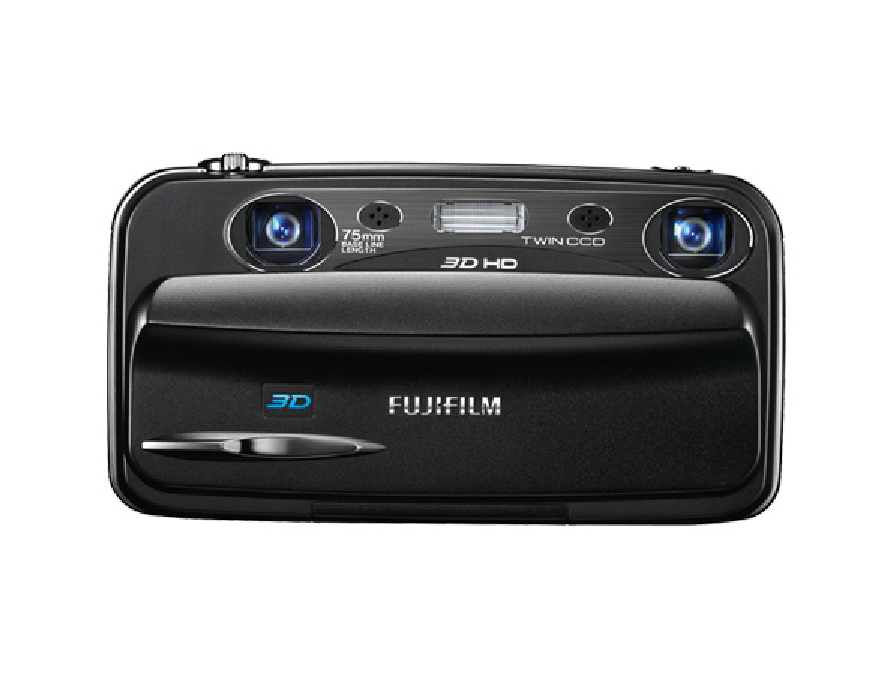
\includegraphics[trim=0.6in 0in 0.4in 0in, clip=true, width=0.3\textwidth]{images/fujifilm.eps}&
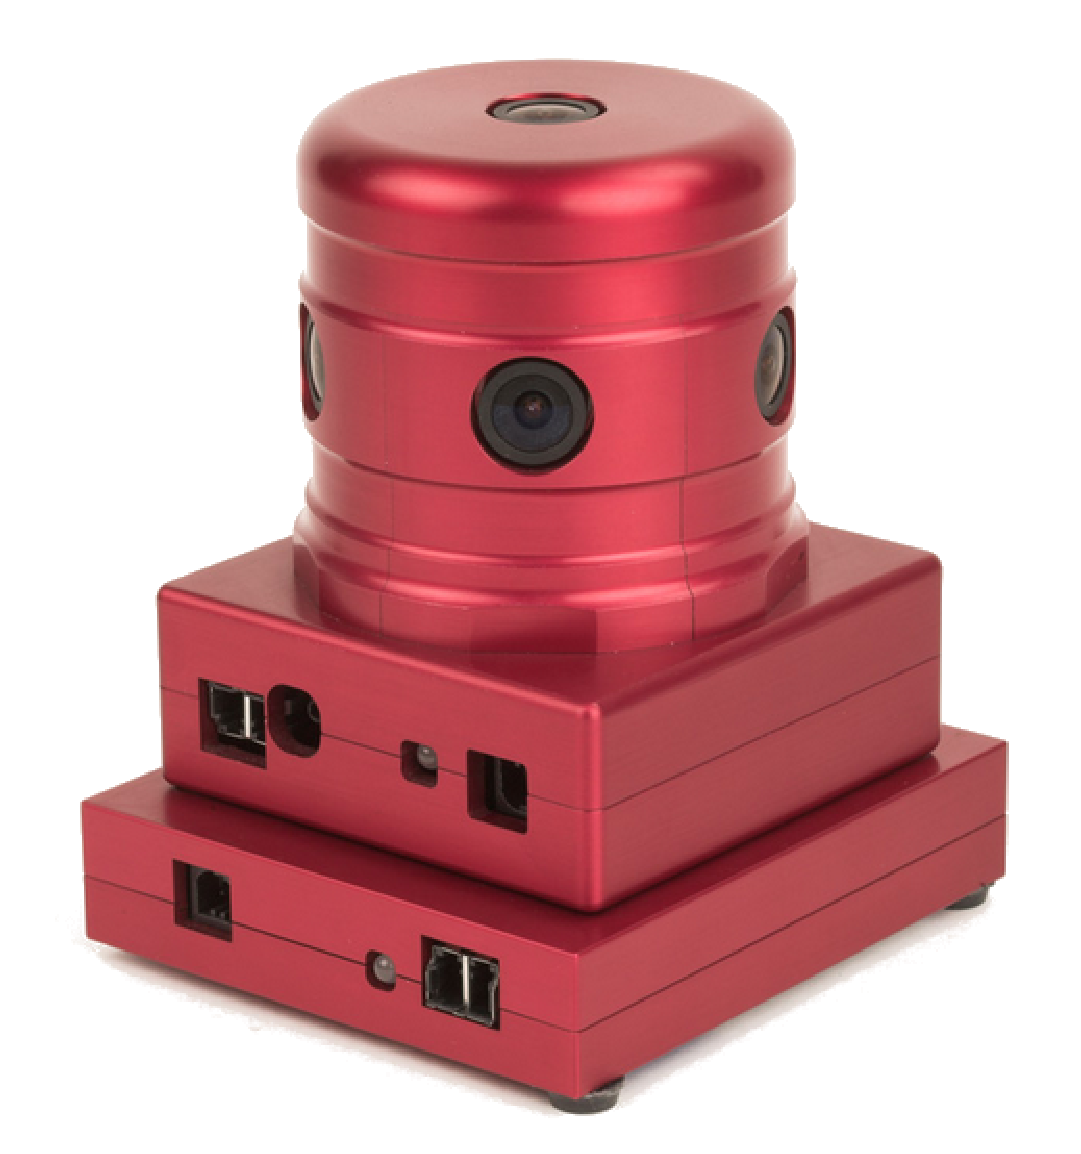
\includegraphics[width=0.27\textwidth]{images/ladybug.eps} & 
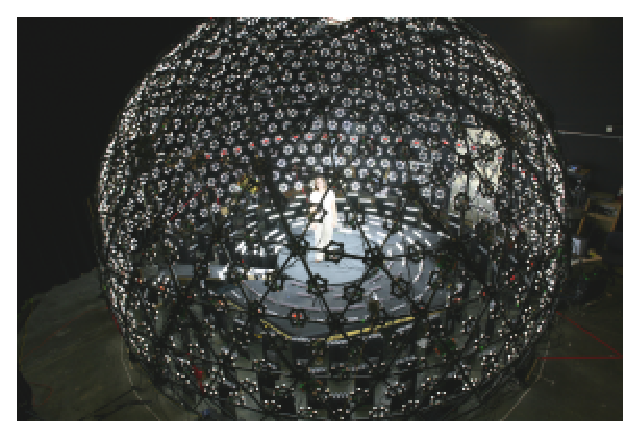
\includegraphics[width=0.4\textwidth]{images/uscSphere.eps} \\
(a) & (b) & (c)
\end{tabular}
\caption{(a) The Fujifilm FinePix Real 3D stereo camera.\protect\footnotemark[1] (b) The Ladybug omnidirectional camera.\protect\footnotemark[2] (c) A multiple camera system for shape capture.\protect\footnotemark[3]}
\label{productFig}
\end{figure}
\end{savenotes}
\footnotetext[1]{Image from \url{http://www.fujifilm.com/}. }
\footnotetext[2]{Image from \url{http://www.ptgrey.com/}. }
\footnotetext[3]{Image from \cite{vlasic2009dynamic}. }

\setlength{\tabcolsep}{4pt}
\begin{figure}
\centering
\begin{tabular}{ccc}
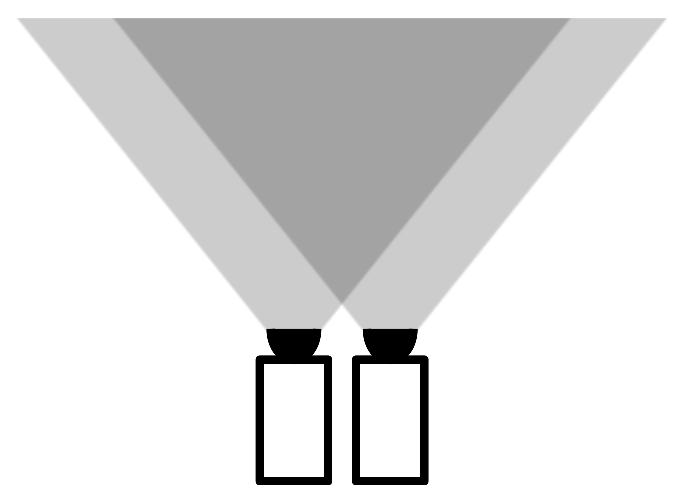
\includegraphics[width=0.3\textwidth]{images/stereofov.eps}&
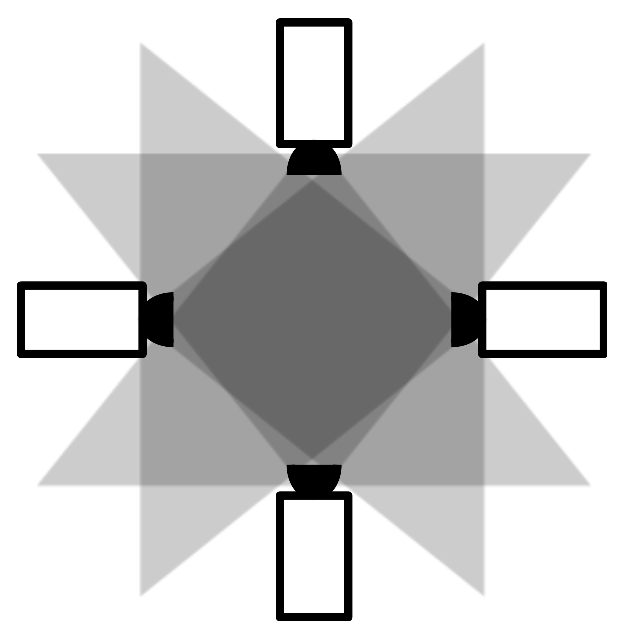
\includegraphics[width=0.3\textwidth]{images/inwardfov.eps}&
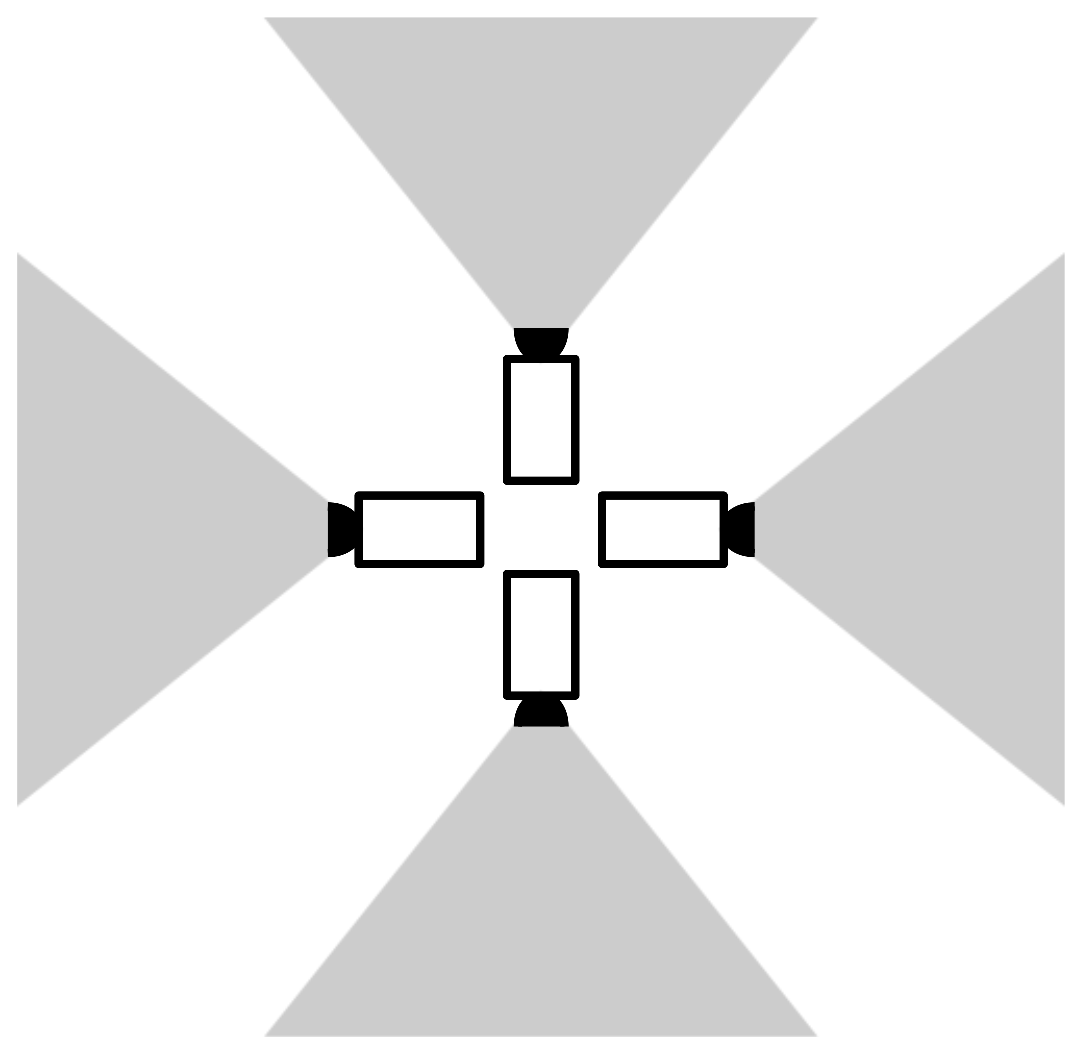
\includegraphics[width=0.33\textwidth]{images/outwardfov.eps}\\
(a) & (b) & (c)
\end{tabular}
\caption{An illustration for the overlapping field of view for different multiple-camera system. The overlapping field of view is plotted as dark region. (a) Stereo camera system, where the two cameras share a large overlapping field of view. (b) Inward looking multiple-camera system, where cameras share a large common field of view. (c) Outward looking multiple-camera system, where cameras share minimal or no common field of view. }
\label{fovFig}
\end{figure}


\subsection{Related Work}
\paragraph{Stereo Camera Calibration} 
The stereo camera system can be easily calibrated using normal calibration pattern such as the chessboard. Figure \ref{fovFig}a shows an illustration of the stereo camera. Since the two neighboring cameras have almost the same field of view, they can capture images of the whole chessboard at the same time. By exploiting the single camera calibration method introduced above in section \ref{singleSec}, the intrinsics of the cameras and the relative pose between the cameras and the chessboard can be estimated. Consider a synchronized pair of images taken by the two cameras for example. If for this pair of images, the relative pose of the first camera is $\mathcal{P}_1$ with respect to the chessboard, and the relative pose of the second camera is $\mathcal{P}_2$ with respect to the chessboard. Then the relative pose between the two cameras can be denoted as $\mathcal{P}_2 \mathcal{P}_1^{-1}$. For multiple pairs of synchronized images, the relative pose can be refined to minimize the summarized reprojection error on all these images. Recent camera calibration toolbox such as \cite{bouguet2004camera, opencv_library} provide available stereo camera calibration functionality. 

\paragraph{Inward-Looking Multiple-Camera System Calibration }
Consder the inward-looking multiple-camera system. From figure \ref{fovFig}b we can see that the cameras in this system share a large overlapping field of view. For some cases where the overlapping field of view is sufficient, the system can be calibrated using the chessboard in a method similar to the stereo camera calibration. For some cases where it is difficult to observe a plane simultaneously by two opposite cameras, some special calibration objects are used for the calibration. For example, in \cite{svoboda2005convenient}, a laser pointer is used as the calibration object. In each set of synchronized images, only one red laser point is detected from each image. A toolbox based on this method is also available. In \cite{kong2013camera}, the authors propose a calibration method using 5 vertical lines, which also performs well for calibrating the inward-looking multiple-camera system. 

\paragraph{Head-Eye Calibration}
Head-eye calibration have been studied for decades in the field of robotics. The head-eye calibration provides a general approach for calibrating the relative pose between any ego-motion sensors. Since the camera motion can be estimated by executing visual odometry estimation, the head-eye calibration technique can also be used to calibrating the extrinsics of a multiple-camera system. Consider a two-camera system for simplicity. By taking synchronized video from the two cameras and executing the visual odometry algorithm, we can obtain the relative ego-motion for the two cameras, denoted as $\mathcal{P}_t^1$ and $\mathcal{P}_t^2$, with $t = 1, 2, \cdots$. Denote the relative pose between the two cameras as $\mathcal{P}$, we have the following constraint: 
\begin{equation}
\mathcal{P}_t^2 = \mathcal{P}^{-1} \mathcal{P}_t^1 \mathcal{P}
\end{equation}
where $t = 1, 2, \cdots$ and $\mathcal{P} \in {SE}(4)$. The head-eye calibration basically aims at solving this equation and obtain $\mathcal{P}$ as the extrinsics between cameras in a multiple-camera system. The accuracy of the head-eye calibration is largely limited by the accuracy of the visual odometry. Since in many cases accurate visual odometry is difficult to obtain, the head-eye calibration can not be widely applied. 

\bigskip
Besides the head-eye calibration method, previous research does not draw much attention on the calibration for the system with its cameras looking outward. As shown in figure \ref{fovFig}c, in the outward-looking camera system cameras have minimal or no overlapping field of view. Due to this limitation, the calibration methods for stereo camera system and inward-looking camera system can not be used for calibrating the outward-looking camera system. We propose our calibration toolbox to solve the calibration problem of outward-looking camera system. 
In this chapter, we based our calibration on the idea of the stereo camera calibration. The difference is that our proposed calibration pattern does not require each pair of cameras to have overlapping field of view. We calibrate the extrinsics between pairs of cameras in the system first and then refine the extrinsics over all cameras. 


\begin{figure}
\centering
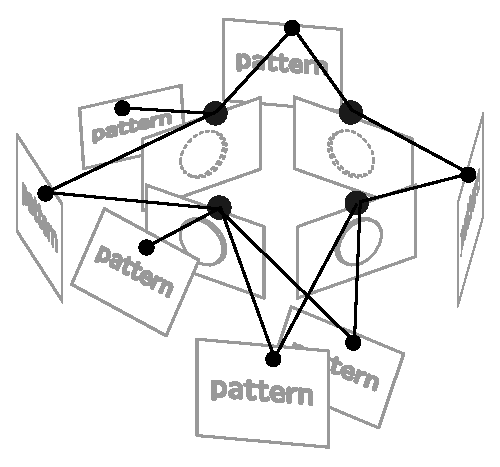
\includegraphics[width=0.6\textwidth]{images/graphsample}
\caption{A example of a pose graph for the calibration scenario of four cameras. Big dots denote camera vertices and small dots denote feature point vertices.}
\label{graphSampleFig}
\end{figure}


\section{Approach}
In our proposed toolbox, we assume that the cameras are rigidly mounted to a rigid body. During the image capture process, we move the calibration pattern around the camera system. From the point correspondences detected from our pattern, we can obtain an estimate for the poses of the calibration pattern by the single camera calibration. If the cameras are synchronized in order to take images of the pattern at the same time, the relative poses of the pattern with respect to each camera are known. Thus, the initial camera poses can be extracted from these relative poses. This procedure is done in the similar way to the extrinsics calibration of the stereo camera. The toolbox then optimizes the initial camera poses using a bundle-adjustment-like method. 

\subsection{Initialization}
We take synchronized images of the pattern by the multiple-camera system. At each timestamp, the calibration pattern is observed by one, two or more cameras. Then the single camera calibration procedure is executed for each camera in the system to firstly estimate the intrinsics and the relative pose between cameras and the pattern. 

Suppose we have $n$ cameras and $m$ timestamps. The $m$ timestamps correspond to $m$ different pose of the calibration pattern with respect to the camera system. We create a pose graph to denote the calibration scenario. Each camera is denoted by a camera vertex $cam_i$, with $i = 1, \dots, n$ in the graph. Meanwhile, each pose of the pattern is also denoted by a pattern vertex $pat_i$, with $i = n + 1, \dots, n + m$. If $cam_i$ takes a photo of the pattern at pose $pat_j$, then $cam_i$ and $pat_j$ are connected by an image edge denoted by $img_{i, j}$. Each edge uniquely corresponds to one image. Note that this graph is a bipartite graph and each edge links one camera vertex and one pattern vertex. Figure \ref{graphSampleFig} provides a simple illustration of such a graph. 

Vertices in the pose graph can be used to store the poses of the cameras and the pattern in a global coordinate system. The global pose of a vertex $i$ is denoted as 
\begin{equation}
\mathcal{P}_{i} = 
\begin{bmatrix}
	\begin{array}{cc}
	\mathbf{R}_{i} & \mathbf{t}_{i} \\ 
	\mathbf{0} & 1
	\end{array}
\end{bmatrix}
\end{equation}
Edges can be used to store the relative pose transform between the camera pose vertex and pattern pose vertex. For each image of the pattern at pose $pat_j$ taken by $cam_i$, we have the relative pose of $pat_j$ with respect to $cam_i$ computed from the single-camera calibration.  The relative pose is denoted as 
\begin{equation}
\mathcal{P}_{i, j} = 
\begin{bmatrix}
	\begin{array}{cc}
	\mathbf{R}_{i, j} & \mathbf{t}_{i, j} \\ 
	\mathbf{0} & 1
	\end{array}
\end{bmatrix}
\end{equation}
where $\mathbf{R}_{i, j}$ and $\mathbf{t}_{i, j}$ are obtained from the single camera calibration

Assuming that the global coordinate system is aligned with the first camera $cam_1$, that is $\mathcal{P}_1 = \mathbf{I}_{4\times4}$, the poses of all vertices connected to $cam_1$ can be obtained by following the image edges from $cam_1$. In practice, if two cameras see the pattern at the same time in their images, then the two cameras are connected via two image edges to one pattern vertex. 

Our toolbox implementation builds a spanning tree with $cam_1$ as its root using breadth-first search on the above pose graph. Vertex poses are then computed by traversing the spanning tree from $cam_1$ and following the image edges. For a edge $img_{i, j}$, if $\mathcal{P}_i$ is known, then $\mathcal{P}_j$ is computed as: 
\begin{equation}
\mathcal{P}_j = \mathcal{P}_i \mathcal{P}_{i, j}
\end{equation} 
Starting from the root $cam_1$, we have initial pose estimates $\mathcal{P}_i$ for all vertices $i = 1, \dots, n + m$ in the global coordinate system.

\subsection{Refinement}
In the initialization stage, we estimate $\mathcal{P}_i$ from $\mathcal{P}_{i, j}$ of $img_{i, j}$ from the spanning tree. In the refinement stage, we re-calculate $\mathcal{P}_{i, j}$ for all edges using $\mathcal{P}_i$. The accuracy of $\mathcal{P}_{i, j}$ can be measured by the reprojection error the image $img_{i, j}$. The reprojection error is denoted as: 
\begin{equation}
\begin{split}
e_{\textrm{reproj}}(\mathbf{X}^w, \mathcal{P}_{i, j}, \mathcal{C}_i) =& \|\hat{\mathbf{m}}(\mathbf{X}^w, \mathcal{P}_{i, j}, \mathcal{C}_i) - \mathbf{m}\|^2 
\end{split}
\end{equation}
where $\hat{\mathbf{m}}(\star)$ is the image projection function corresponding to camera $cam_i$. $\mathcal{C}_i$ denotes all the intrinsic parameters of camera $cam_i$. 

The initial calibration estimate is refined to minimize the summation of all reprojection errors. The refinement can be over either all vertex poses or over both vertex poses and intrinsics. The optimization problem with only vertex poses is defined as: 
\begin{equation}
\begin{aligned}
& \argmin_{\mathcal{P}_i, i > 1} & & \sum_{img_{i, j}} \sum_{\mathbf{X}^w} e_{\textrm{reproj}}(\mathbf{X}^w, \mathcal{P}_i^{-1} \mathcal{P}_j, \mathcal{C}_i) 
\end{aligned}
\end{equation}
where we use the fact that $\mathcal{P}_{i, j} = \mathcal{P}_i^{-1} \mathcal{P}_j$. The optimization on $\mathcal{P}_i$ is over the 6-DoF space of $SE(4)$. In the implementation of our toolbox, $\mathcal{P}_i$ is parametrized as rotation and translation. The rotation is then parametrized using the angle-axis denotion. 
The optimization problem with both vertex poses and intrinsics is denoted as: 
\begin{equation}
\begin{aligned}
& \argmin_{\mathcal{P}_i, \mathcal{C}_1, \mathcal{C}_i, i > 1} & & \sum_{img_{i, j}} \sum_{k} e_{\textrm{reproj}}(\mathbf{X}^w, \mathcal{P}_i^{-1} \mathcal{P}_j, \mathcal{C}_i)
\end{aligned}
\end{equation}
Note both optimization is over $\mathcal{P}_i$ with $i > 1$, since $\mathcal{P}_1 \equiv \mathbf{I}_{4 \times 4}$ is the world frame. The toolbox executes the optimization using the Levenberg-Marquardt algorithm. 

The refinement of the extrinsic calibration is analogous to the bundle adjustment in the research of structure from motion (SfM) and visual odometry. Especially, if camera vertices are connect in a loop in the pose graph, the refinement can significantly improve the calibration result, similarly to the loop closure procedure in visual odometry. 


\chapter{Experiments}
We carry out two experiments with our proposed calibration pattern and toolbox. In the first experiment, we use a stereo camera and compare the calibration results from our toolbox and those from the OpenCV-based chessboard calibration. In the second and third experiment, we use our toolbox to calibrate a four-camera system and a five-camera system respectively. The latter two camera systems are especially challenging for existing multiple-camera calibration methods. 

\begin{figure}
\centering
%\begin{tabular}{cc}
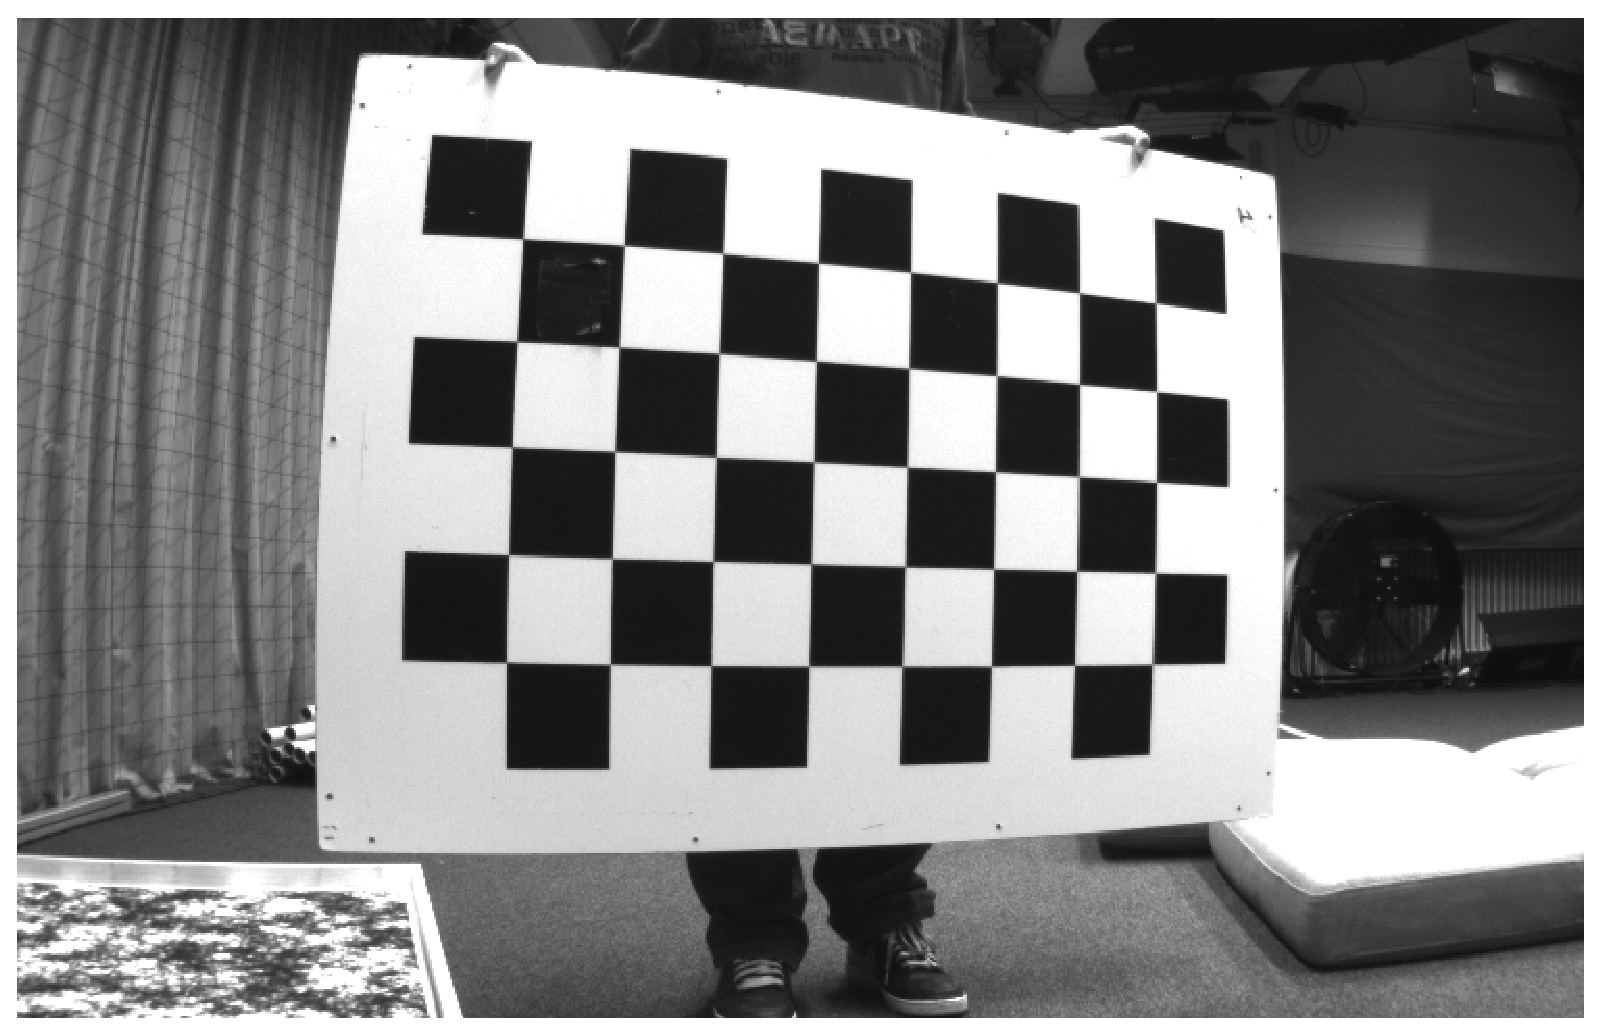
\includegraphics[width=0.49\textwidth]{images/left000} 
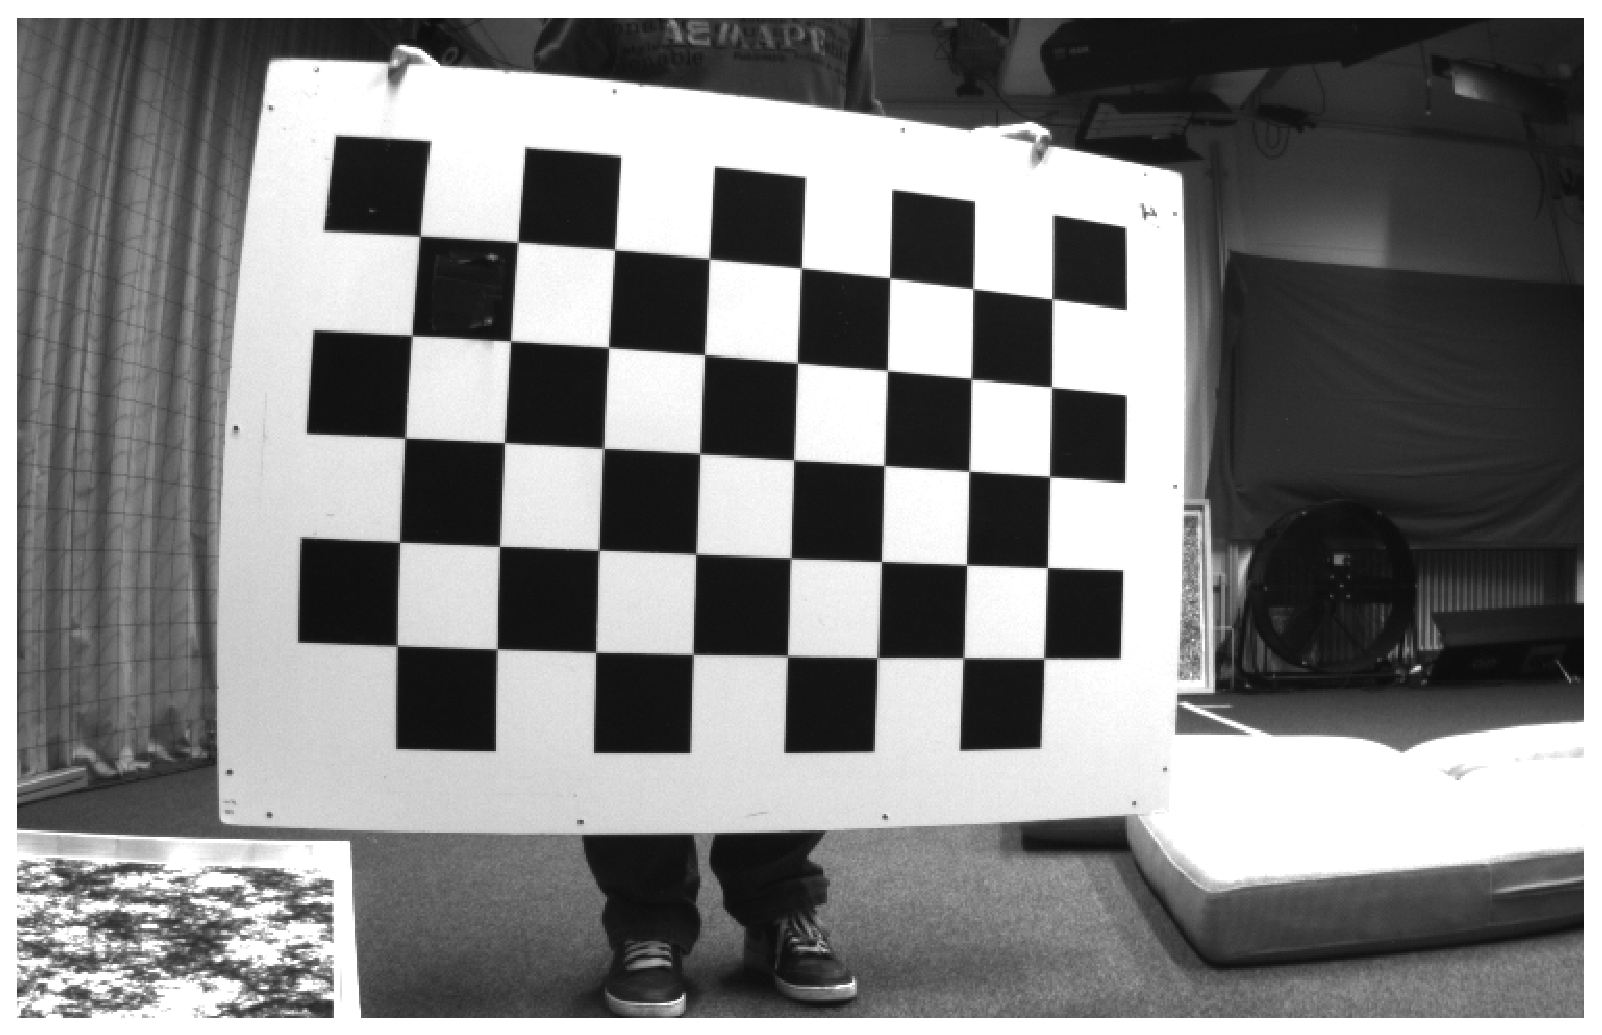
\includegraphics[width=0.49\textwidth]{images/right000} \\ 
\vspace{3pt}
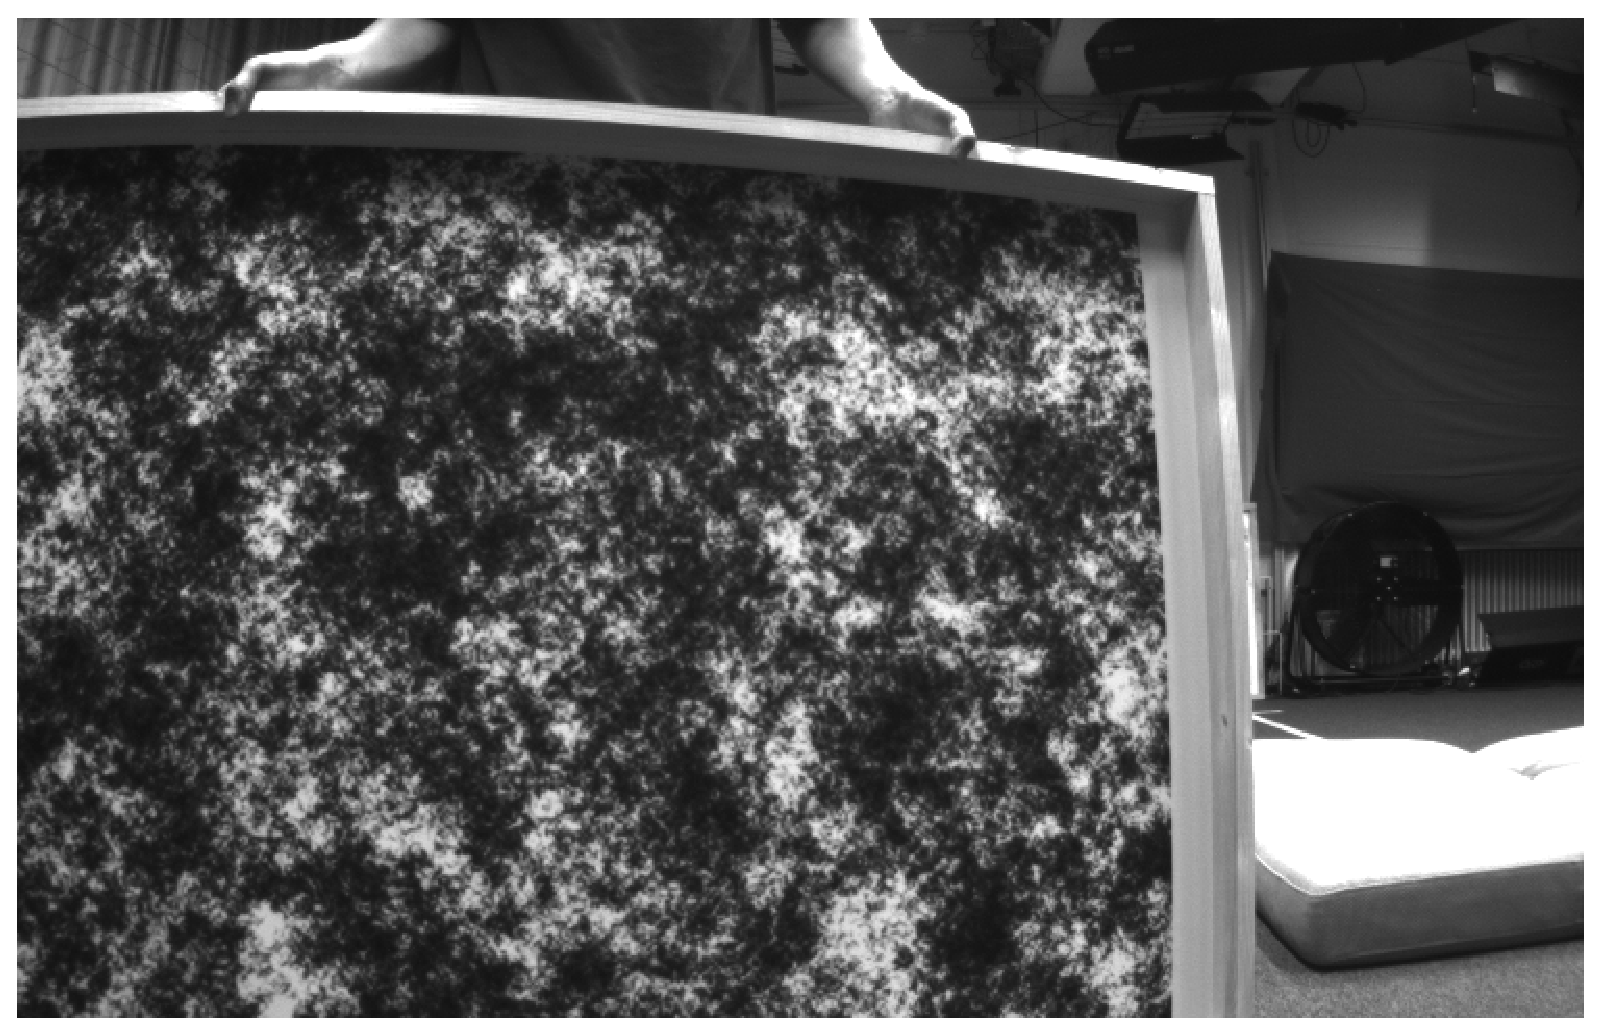
\includegraphics[width=0.49\textwidth]{images/left001} 
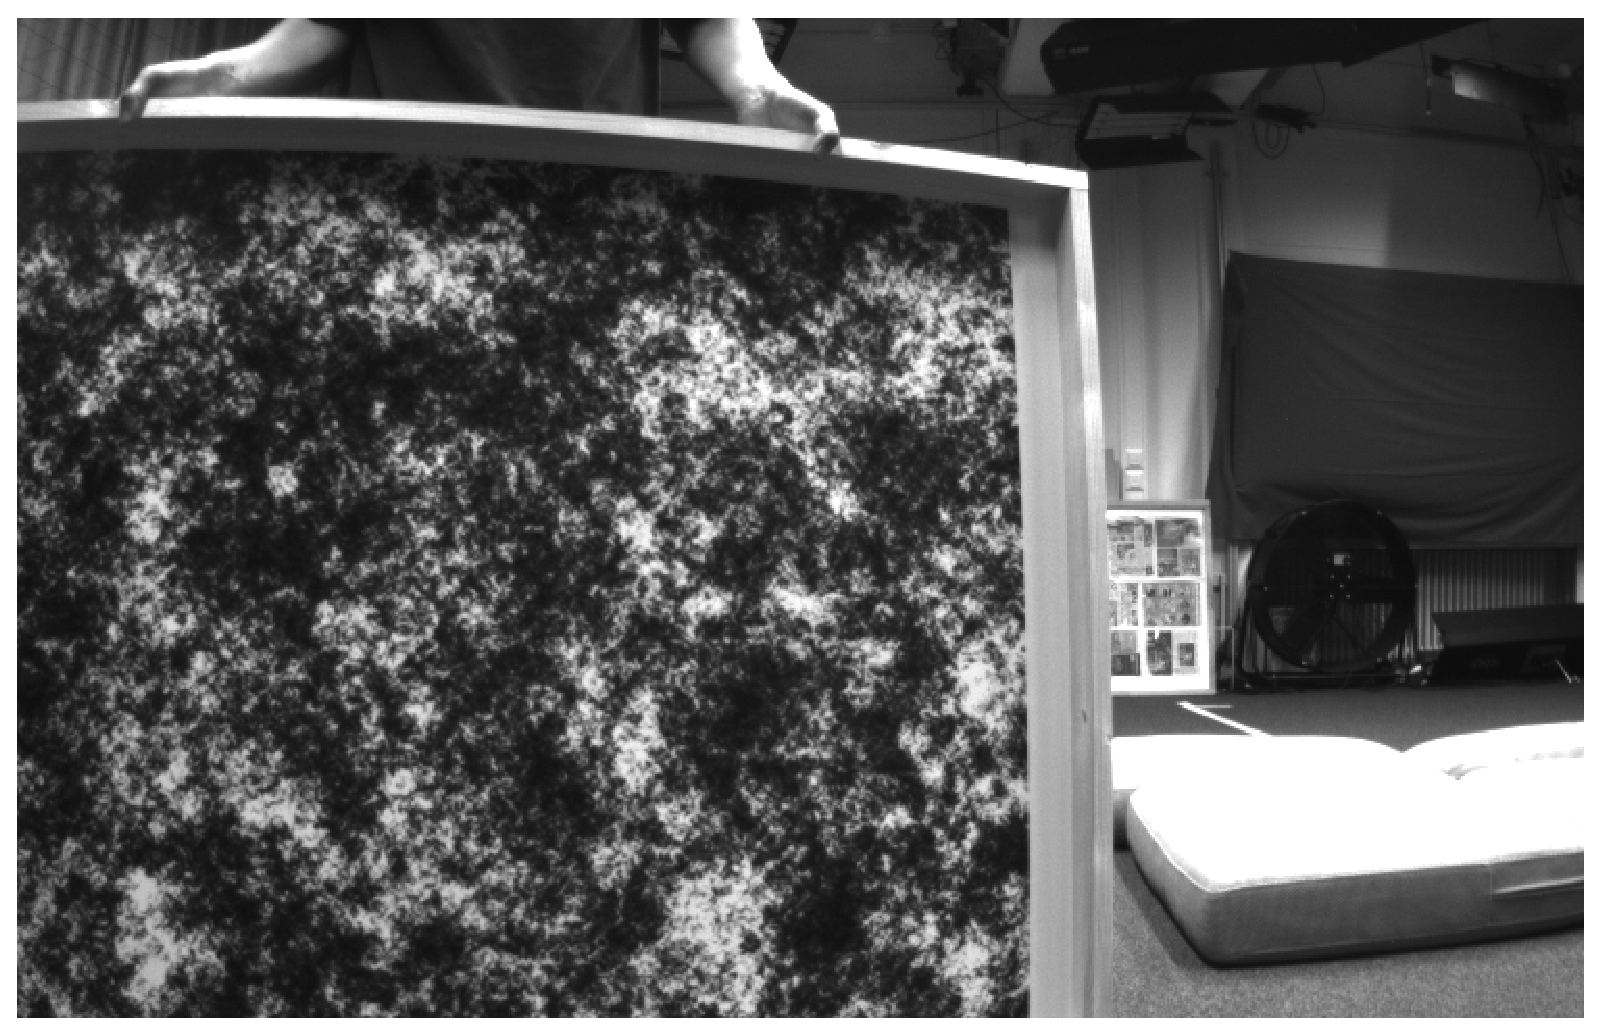
\includegraphics[width=0.49\textwidth]{images/right001} 
%\end{tabular}
\caption{Sample images used to calibrate the stereo camera. The top row shows a chessboard used by the chessboard calibration while the bottom row shows our calibration pattern used by our calibration toolbox. }
\label{stereoImageFig}
\end{figure}



\begin{figure}
\centering
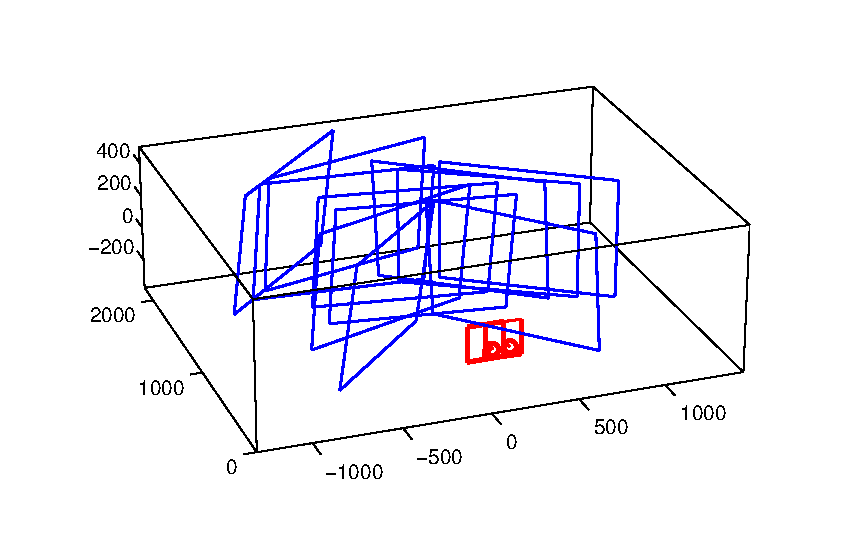
\includegraphics[trim=0in 0.1in 0in 0in, clip=true, width = 0.7\textwidth]{images/stereo3dbold}
\caption{3D plot of stereo camera and calibration pattern poses generated by our toolbox.}
\label{stereoPlot}
\end{figure}

\begin{table}
\centering
\begin{tabular}{|c|c|c|}
\hline
Object & Descriptor-based pattern & $5 \times 8$ chessboard \\
\hline
\begin{tabular}{c}
Image 
size
\end{tabular} & $480 \times 752$ & $480 \times 752$ \\[4pt]
\hline
{\#} images & $10 \times 2$ & $30 \times 2$\\
\hline
\begin{tabular}{c}
{\#} features \\
(L/R)
\end{tabular} & 3073 / 2942 & 1200 / 1200 \\
\hline
\begin{tabular}{c}
Focal \\
length (L)
\end{tabular} & $(720, 718)$ & $(720, 722)$ \\
\hline
\begin{tabular}{c}
Focal \\
length (R)
\end{tabular} & $(709, 706)$ & $(709, 710)$ \\
\hline
\begin{tabular}{c}
Principal \\
point (L)
\end{tabular} & $(383, 249)$ & $(392, 250)$ \\
\hline
\begin{tabular}{c}
Principal \\
point (R)
\end{tabular} & $(387, 242)$ & $(389, 249)$ \\
\hline
\begin{tabular}{c}
Rotation \\
vector
\end{tabular} & $\left[0.001, -0.010, 0.011\right]$ & $\left[0.004, -0.009, 0.011\right]$ \\
\hline
\begin{tabular}{c}
Translation\\
vector (unit)
\end{tabular} & $\left[-1.00, -0.012, 0.005\right]$ & $\left[-1.00, -0.011, 0.012\right]$ \\
\hline
\begin{tabular}{c}
Reprojection \\
error 
\end{tabular} & 0.4 px & 0.2 px \\
\hline
\end{tabular}
\caption{Comparison of results from our method and OpenCV-based chessboard calibration for a stereo camera.}
\label{comparisonTab}
\end{table}

\section{Calibration of a Stereo Camera}
For the case of a stereo camera, a chessboard is typically used for extrinsic calibration. The two cameras tend to have a large overlapping field of view, and the entire chessboard has to be in both cameras' fields of view. We test our toolbox with a custom-built stereo camera comprising two mvBlueFOX cameras with hardware synchronization. Figure \ref{stereoImageFig} shows a sample stereo image pair used for each calibration. Note that in contrast to the chessboard calibration, our proposed calibration pattern does not have to be entirely within the field of view. The calibration results are shown in table \ref{comparisonTab}. The descriptor-based pattern provides many more features with significantly fewer images compared to the chessboard pattern. We observe that the two calibration results are very similar. The reprojection error for our proposed pattern is higher than that for the chessboard. This is because SURF feature detection is slightly less accurate than sub-pixel chessboard corner detection in terms of feature location. For features on a coarser scale, the higher corresponding error of the estimated feature coordinates may increase the overall reprojection error. We visualize the results of our toolbox calibration in figure \ref{stereoPlot}.

\setlength{\tabcolsep}{2pt}
\begin{figure}
\centering
\begin{tabular}{cc}
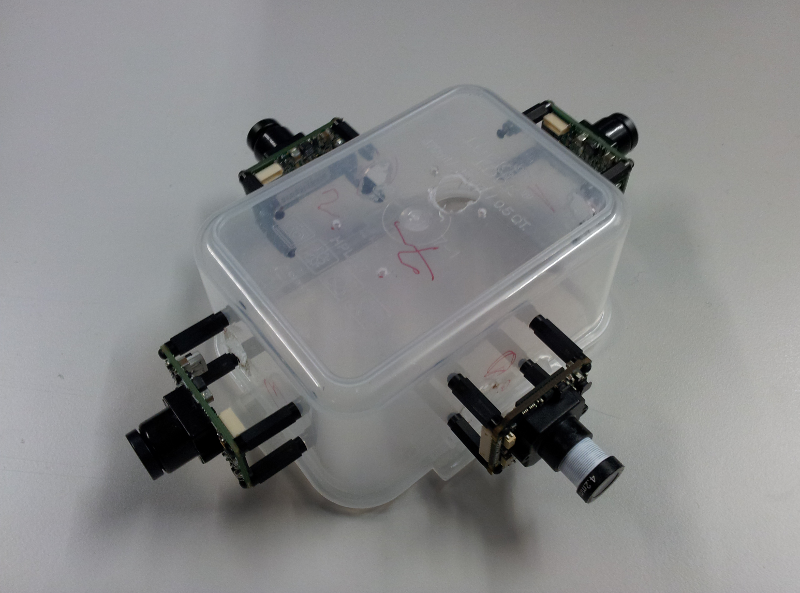
\includegraphics[width=0.574\textwidth]{images/fourcamerarig}&
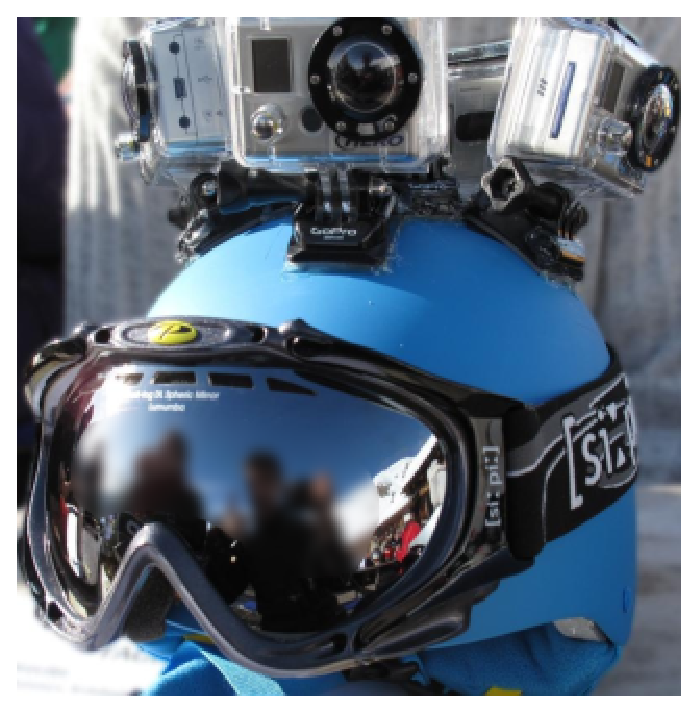
\includegraphics[width=0.416\textwidth]{images/helmet} \\
(a) & (b)
\end{tabular}
\caption{A four-camera system with an approximate 90\ensuremath{^\circ} relative rotation between each pair of neighboring cameras.}
\label{cameraRigPhoto}
\end{figure}


\begin{figure}
\centering
%\begin{tabular}{cc}
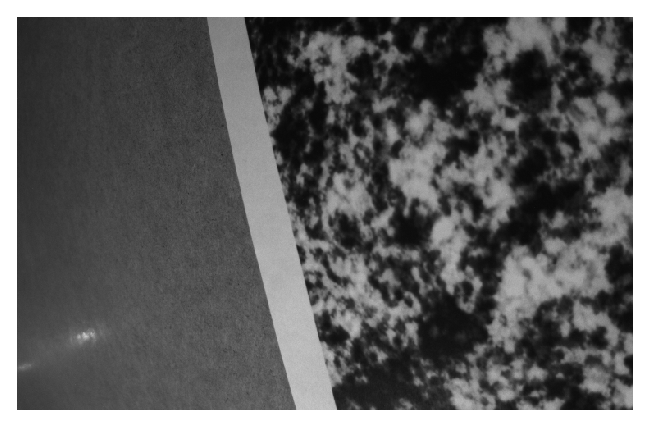
\includegraphics[width=0.27\textwidth]{images/cam4rig/1} 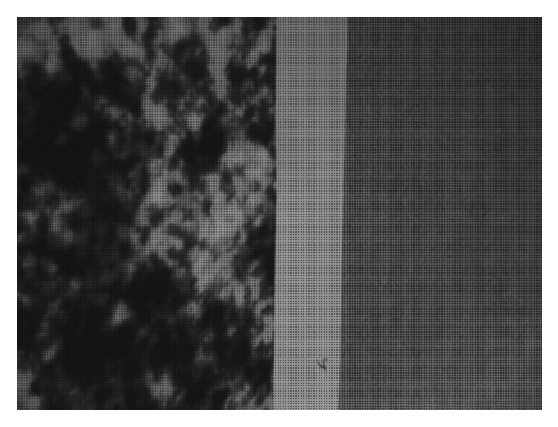
\includegraphics[width=0.23\textwidth]{images/cam4rig/2} \hspace{0.5pt}
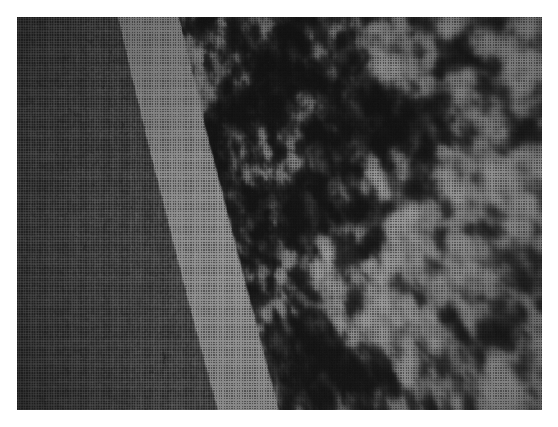
\includegraphics[width=0.23\textwidth]{images/cam4rig/3}
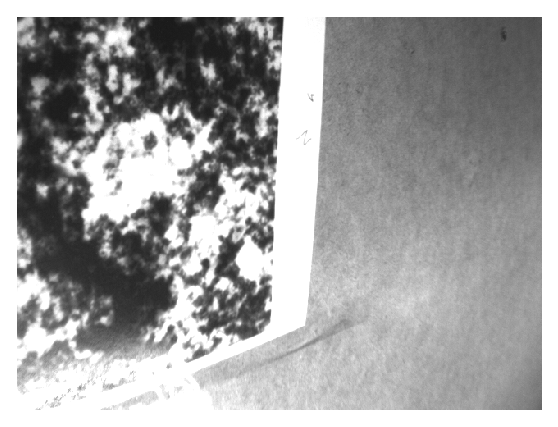
\includegraphics[width=0.23\textwidth]{images/cam4rig/4} \\
\vspace{5pt}
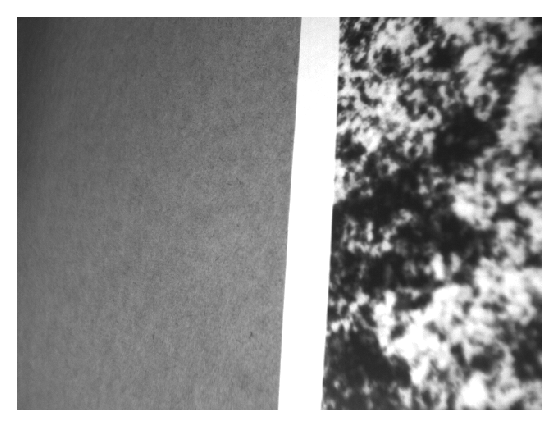
\includegraphics[width=0.23\textwidth]{images/cam4rig/5} 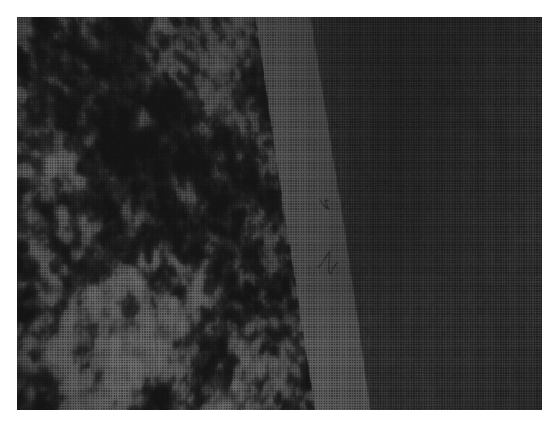
\includegraphics[width=0.23\textwidth]{images/cam4rig/6} \hspace{0.5pt}
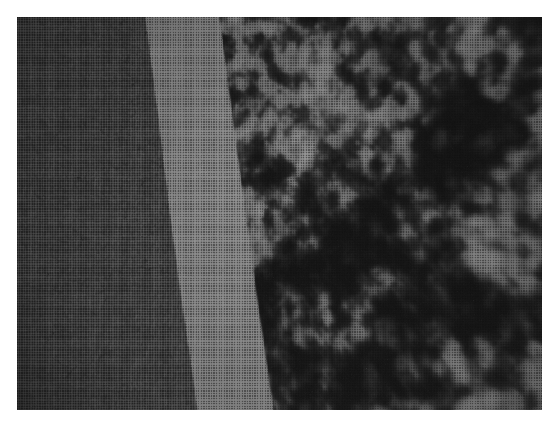
\includegraphics[width=0.23\textwidth]{images/cam4rig/7}
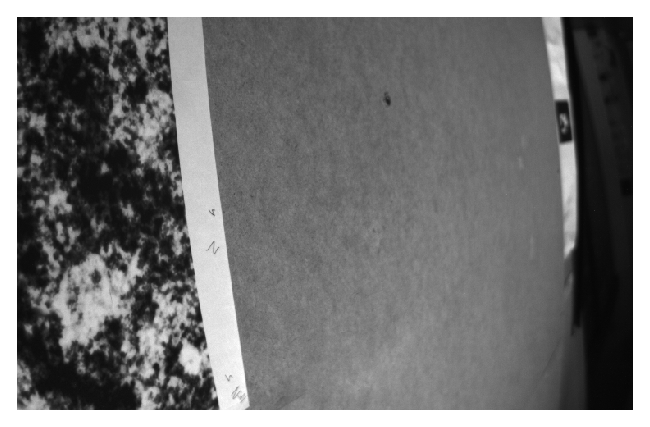
\includegraphics[width=0.27\textwidth]{images/cam4rig/8} \\%\end{tabular}
\caption{Sample images used to calibrate the four-camera rig. Each pair corresponds to an image pair from a different pair of neighboring cameras. Top-left: camera 1 and camera 2. Top-right: camera 2 and camera 3. Bottom-left: camera 3 and camera 4. Bottom-right: camera 4 and camera 1. Note that camera 1 has different resolution with the other three cameras. }
\label{cameraRigImageFig}
\end{figure}

\begin{figure}
\centering 
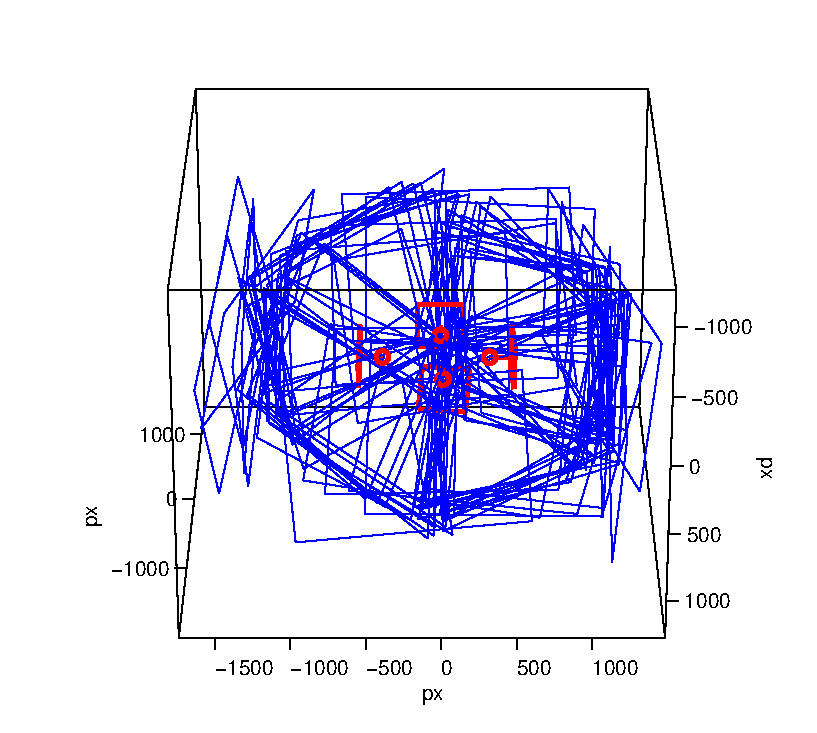
\includegraphics[trim=1in 0in 0.1in 0.4in, clip=true, width=0.47\textwidth]{images/rig2} 
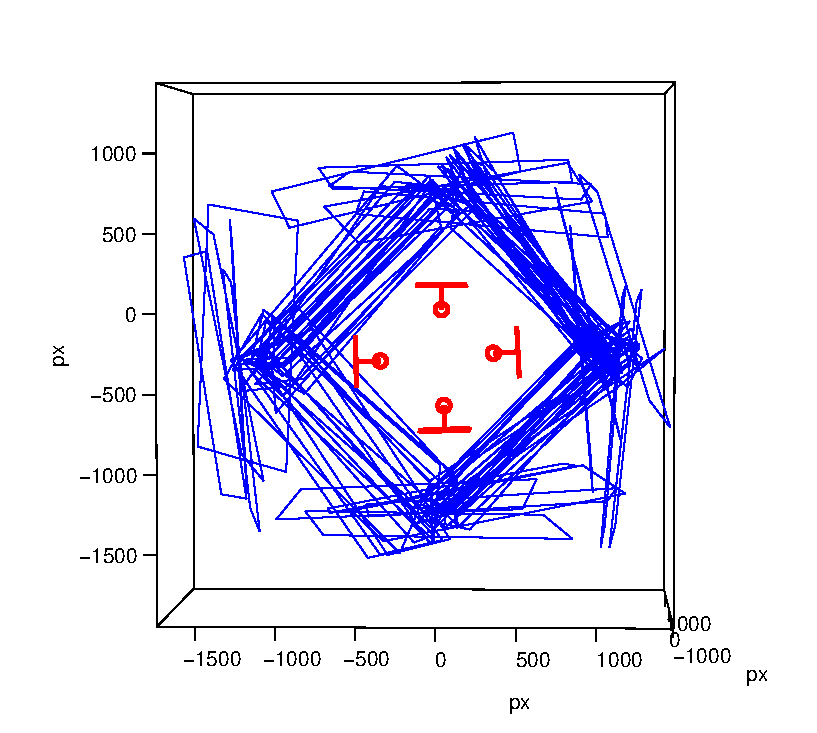
\includegraphics[trim=0.2in 0in 0.6in 0.4in, clip=true, width=0.5\textwidth]{images/rig1} 
\caption{Two viewpoints of a 3D plot of camera and calibration pattern poses generated by our toolbox for the 4-camera system. } 
\label{cameraRigPlot}
\end{figure}



\section{Calibration of a Four-Camera System}
In the second experiment, we validate our toolbox on a four-camera system; neighboring cameras have minimal overlapping fields of view. One camera is a mvBlueFOX camera while the rest are Point Grey Firefly MV cameras. This system is shown in figure \ref{cameraRigPhoto}a. The cameras are synchronized by hardware. All the four cameras are normal pinhole cameras. Existing camera calibration toolboxes are difficult to use when it comes to calibrating such systems. 15 image pairs are taken for each pair of neighboring cameras; two examples are shown in figure \ref{cameraRigImageFig}a. Due to the non-overlapping field of view, neighboring cameras only see a small part of the board close to the board's border. Thus, some images do not have sufficient features for matching, and are automatically discarded by the toolbox. In addition, to ensure accurate intrinsic calibration, we take 5 images for each camera with the pattern occupying a large part of each image. Figure \ref{cameraRigPlot} plots the 3D poses of both cameras and patterns. The average reprojection error over all images and corresponding to the estimated intrinsics and extrinsics is $0.7$ pixels. 

%\begin{figure}
%\centering 
%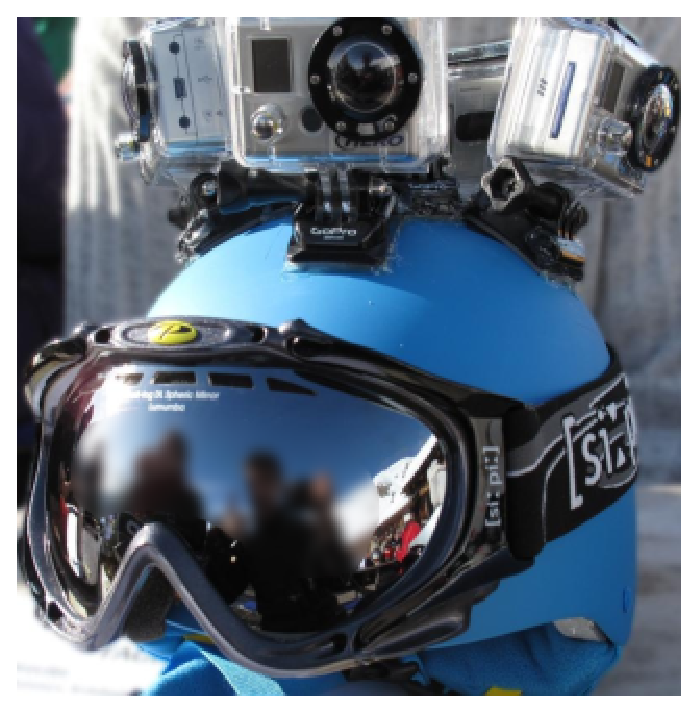
\includegraphics[width=0.57\textwidth]{images/helmet} 
%\caption{A 5-camera system mounted on a ski helmet}. 
%\label{helmetPhoto}
%\end{figure}

\begin{figure*}
\centering
%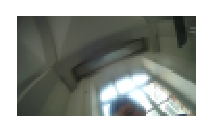
\includegraphics[width=0.115\textwidth]{images/sampleimage/9-1} 
%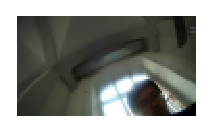
\includegraphics[width=0.115\textwidth]{images/sampleimage/32-1} 
%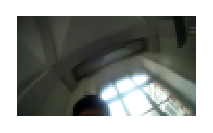
\includegraphics[width=0.115\textwidth]{images/sampleimage/48-1} 
%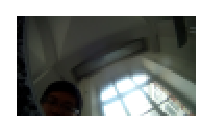
\includegraphics[width=0.115\textwidth]{images/sampleimage/67-1} 
%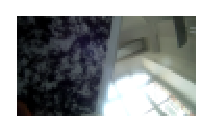
\includegraphics[width=0.115\textwidth]{images/sampleimage/125-1} 
%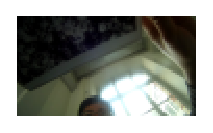
\includegraphics[width=0.115\textwidth]{images/sampleimage/155-1} 
%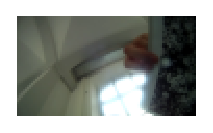
\includegraphics[width=0.115\textwidth]{images/sampleimage/197-1} 
%\includegraphics[width=0.115\textwidth]{images/sampleimage/204-1} \\ \vspace{4pt}
\includegraphics[width=0.115\textwidth]{images/sampleimage/9-2} 
\includegraphics[width=0.115\textwidth]{images/sampleimage/32-2} 
\includegraphics[width=0.115\textwidth]{images/sampleimage/48-2} 
\includegraphics[width=0.115\textwidth]{images/sampleimage/67-2} 
\includegraphics[width=0.115\textwidth]{images/sampleimage/125-2} 
\includegraphics[width=0.115\textwidth]{images/sampleimage/155-2} 
\includegraphics[width=0.115\textwidth]{images/sampleimage/197-2} 
\includegraphics[width=0.115\textwidth]{images/sampleimage/204-2} \\ \vspace{4pt}
\includegraphics[width=0.115\textwidth]{images/sampleimage/9-3.eps} 
\includegraphics[width=0.115\textwidth]{images/sampleimage/32-3} 
\includegraphics[width=0.115\textwidth]{images/sampleimage/48-3} 
\includegraphics[width=0.115\textwidth]{images/sampleimage/67-3} 
\includegraphics[width=0.115\textwidth]{images/sampleimage/125-3} 
\includegraphics[width=0.115\textwidth]{images/sampleimage/155-3} 
\includegraphics[width=0.115\textwidth]{images/sampleimage/197-3} 
\includegraphics[width=0.115\textwidth]{images/sampleimage/204-3} \\ \vspace{4pt}
\includegraphics[width=0.115\textwidth]{images/sampleimage/9-4} 
\includegraphics[width=0.115\textwidth]{images/sampleimage/32-4} 
\includegraphics[width=0.115\textwidth]{images/sampleimage/48-4} 
\includegraphics[width=0.115\textwidth]{images/sampleimage/67-4} 
\includegraphics[width=0.115\textwidth]{images/sampleimage/125-4} 
\includegraphics[width=0.115\textwidth]{images/sampleimage/155-4} 
\includegraphics[width=0.115\textwidth]{images/sampleimage/197-4} 
\includegraphics[width=0.115\textwidth]{images/sampleimage/204-4} \\ \vspace{4pt}
\includegraphics[width=0.115\textwidth]{images/sampleimage/9-5} 
\includegraphics[width=0.115\textwidth]{images/sampleimage/32-5} 
\includegraphics[width=0.115\textwidth]{images/sampleimage/48-5} 
\includegraphics[width=0.115\textwidth]{images/sampleimage/67-5} 
\includegraphics[width=0.115\textwidth]{images/sampleimage/125-5} 
\includegraphics[width=0.115\textwidth]{images/sampleimage/155-5} 
\includegraphics[width=0.115\textwidth]{images/sampleimage/197-5} 
\includegraphics[width=0.115\textwidth]{images/sampleimage/204-5} \\ \vspace{4pt}
\includegraphics[width=0.115\textwidth]{images/sampleimage/9-6} 
\includegraphics[width=0.115\textwidth]{images/sampleimage/32-6} 
\includegraphics[width=0.115\textwidth]{images/sampleimage/48-6} 
\includegraphics[width=0.115\textwidth]{images/sampleimage/67-6} 
\includegraphics[width=0.115\textwidth]{images/sampleimage/125-6} 
\includegraphics[width=0.115\textwidth]{images/sampleimage/155-6} 
\includegraphics[width=0.115\textwidth]{images/sampleimage/197-6} 
\includegraphics[width=0.115\textwidth]{images/sampleimage/204-6} 
\caption{Sample images used for calibrating the helmet-mounted five-camera system. Each row corresponds to images from an unique camera. Each column corresponds to images with a common timestamp. }
\label{helmetImageFig}
\end{figure*}

\begin{figure}
\centering 
\includegraphics[trim=0.4in 0in 0.4in 0.0in, clip=true, width=0.47\textwidth]{images/5rig2} 
\includegraphics[trim=0.1in 0in 0.4in 0.5in, clip=true, width=0.52\textwidth]{images/5rig1} 
\caption{Two viewpoints of a 3D plot of camera and calibration pattern poses generated by our toolbox for the 5-camera system. } 
\label{fiveCameraRigPlot}
\end{figure}

\section{Calibration of a Five-Camera System}
The the third experiment, we validate our toolbox on a five-camera system made up of wide angle cameras. The cameras are mounted as a rig on a ski helmet, as is shown in figure \ref{cameraRigPhoto}b. The cameras are five GoPro 2 cameras, under wide angle mode. We take 5 videos from the cameras of a moving calibration pattern. The videos are then synchronized by aligning the audio signal. Figure \ref{cameraRigPhoto}b shows some sample images take from the videos. Each row corresponds to one camera. Each column corresponds to one timestamp after synchronization. The generic camera model is used for single camera calibration. Figure \ref{fiveCameraRigPlot} plots the 3D poses of both cameras and patterns. 

\chapter{Some Explorations on Calibration Using a LCD Display}
The flat screen and good brightness quality of LCD displays is very suitable for displaying calibration pattern. In this part, we show some explorations on using LCD displays for calibration. The main idea of exploiting a LCD display in calibration is to achieve more correspondences in calibration. 

In general, more correspondences result in more accurate and stabler calibration result. Calibration patterns such as chessboard or our features-based pattern usually provide no more than 1000 correspondences. In some recent study, researchers propose some techniques of generating much denser correspondences in calibration.  For example, \cite{grosse2012camera, schmalz2011camera} use temporal code for indexing points on a display and can achieve very dense correspondences. This technique is not very convenient as it requires the camera to be fixed on tripod and take video at different poses to percept the entire temporal code. 

Another aspect to achieve dense correspondences is to render the reprojected calibration pattern and compare it with the original pattern. \cite{schiller2008calibration} has done some similar work using chessboard pattern. To render a reprojected calibration pattern, we firstly calibrate the camera using normal correspondences like chessboard corners. Thus the camera intrinsics as the chessboard pose are both known. Then the chessboard photo can be reprojected back to the pattern plane. The reprojected pattern is very similar to the original pattern, with only small deviation or difference due to the initial calibration precision. Thus we have a pixel-wise correspondence between the two images. It is then possible to refine the calibration result by minimizing the summation of pixel-wise difference, such as SSD or SAD, between the reprojected pattern and the original pattern. 

In this chaper, we mainly focus on this above aspect of refining calibration by minimizing the SSD between the original pattern and the reprojected pattern. First we provide a formulation of the refinement problem. For a point $\mathbf{X}^w = [X^w, Y^w, 0]^\top$ on the calibration pattern, its corresponding image point $\hat{\mathbf{m}}(\mathbf{X}^w, \mathbf{R}, \mathbf{t}, \mathcal{C})$ can be obtained via equations \ref{cmEqn1}, \ref{rayEqn}, \ref{distEqn0}, and \ref{cmEqn4}. We assume that $\mathbf{X}^w = [X^w, Y^w, 0]^\top$ is measured by pixel. Denote $\mathbf{I}_p$ as image of the calibration pattern. Thus the $\mathbf{I}_p(X^w, Y^w)$ denotes the grayscale of the calibration pattern at the pixel $\mathbf{X}^w = [X^w, Y^w, 0]^\top$. The SSD between reprojected pattern and the original pattern is: 
\begin{equation}
SSD_{\mathbf{I}_p}(\mathbf{I}_\text{im}) = \sum_{X^w, Y^w} \left\|\mathbf{I}_p(X^w, Y^w) - \mathbf{I}_\text{im}(\hat{\mathbf{m}}(\mathbf{X}^w, \mathbf{R}, \mathbf{t}, \mathcal{C}))\right\|^2
\end{equation}
where $\mathbf{I}_p$ is the original pattern image and $\mathbf{I}_\text{im}$ is a photo of the pattern. Thus the refinement stage can be formed as: 
\begin{equation}
\min_{\mathbf{R}_i, \mathbf{t}_i, \mathcal{C}, \forall i} \sum_{i} SSD_{\mathbf{I}_p}(\mathbf{I}_\text{im}^i)
\label{SSDObjEqn}
\end{equation}
where $i$ is the index of each image. $\mathcal{C}$ denotes all the camera intrinsic parameters. 

The above equation provides a simple formulation for refining the calibration result by comparing grayscale between all the pixels in the original pattern and the reprojected pattern. Note that in general the grayscale difference between the original pattern and the reprojected pattern is caused by two factors: One is the misalignment of pixels due to the inaccuracy of calibration; The other is the non-linear grayscale conversion from image data to the display output response and from the display output to the photo data. The above equation only considers the first factor of inaccuracy of calibration. To consider the second factor, we add a grayscale conversion function $f(x, \star)$ to denote the non-linear grayscale conversion. Thus the SSD is modified as: 
\begin{equation}
SSD_{\mathbf{I}_p}(\mathbf{I}_\text{im}) = \sum_{X^w, Y^w} \left\| f\left( \mathbf{I}_p(X^w, Y^w), \star \right) - \mathbf{I}_\text{im}\left(\hat{\mathbf{m}}(\mathbf{X}^w, \mathbf{R}, \mathbf{t}, \mathcal{C})\right)\right\|^2\label{newSSDEqn}
\end{equation}
Note that we put a $\star$ in $f$ because the function value is also determined by other factors, which will be discussed next. 

\begin{figure}
\centering
\includegraphics[width=0.9\textwidth, trim=0.5in 7in 1.5in 0in, clip=true]{images/render-flow-chart.pdf}
\caption{A flowchart of the refining the calibration by minimizing the SSD between the original pattern and the reprojected pattern. The original calibration pattern image (top-left) is shown on a display and captured by a camera as a photo (top-right). The photo is then reprojected back to the calibration pattern plane (bottom-right).  Meanwhile, the grayscale of the original calibration pattern image is converted according to the response function of the display. The converted pattern image (bottom-left) is the compared with the reprojected photo (bottom-right) to refine the camera parameters. The top-left original pattern image corresponds to figure \ref{displayPattern}a; The top-right captured photo corresponds to figure \ref{displayPattern}b; The bottom-left converted pattern image corresponds to figure \ref{displayPattern}f; The bottom-right reprojected image corresponds to figure \ref{displayPattern}c.} 
\label{displayFlow}
\end{figure}

Figure \ref{displayFlow} shows a flowchart of how the refinement works. See the figure caption for illustrations. Note that the camera sensor response is not consider since we use the RAW image in our experiment, as will be stated next. 

\section{Explorations on Estimating the Display Output Response}

\begin{figure}
\centering
\begin{tabular}{ccc}
\includegraphics[width=0.3\textwidth]{images/display-pattern.png}&
\includegraphics[width=0.343\textwidth]{images/display-photo.png}&
\includegraphics[width=0.3\textwidth]{images/rendered.png}\\
(a) & (b) & (c)
\end{tabular}
\begin{tabular}{ccc}
\includegraphics[width=0.3\textwidth]{images/rendered-sample.png}&
\includegraphics[width=0.3\textwidth]{images/fitted-gray.png}&
\includegraphics[width=0.3\textwidth]{images/fitted-image.png}\\
(d)&(e)&(f)
\end{tabular}
\caption{(a) An original calibration pattern with noise tiles and solid tiles. (b) A raw image photo of the pattern on a display. The RAW image grayscale value is scaled for visualization. (c) The reprojected pattern of (b) on the pattern plane. (d) Enroded solid tiles of grayscale-255 extracted from (c). (e) An visualization of the display grayscale response for grayscale-255 in image (b). This can be interpreted as an interpolation of tile grayscales in (d). (f) A pattern generated from the original pattern by converting its grayscale according to the display grayscale response. }
\label{displayPattern}
\end{figure}

The active-matrix liquid-crystal display (AMLCD) is the current mostly used computer display techniques, on either notebooks or desktops. The AMLCD is advantageous for its low weight, good image quality, wide color gamut and good response time. The narrow viewing angle is one of the drawbacks for all LCD techniques. The displays have the best brightness when viewing in its front. When viewing from side, the brightness will be very low. 

We base our study on normal desktop display of AMLCD. In our study, we assume that on the display, all pixels are ideally the same and the background light is uniform. Thus the brightness of each pixel is only determined by the input image grayscale and the viewing angle. 

We show here a experiment of estimating the display response $f(g, \star)$ for different input grayscale value $g$. Three variables are considered: the horizontal viewing angle, the vertical viewing angle and the input grayscale. Thus the $\star$ in the $f$ function in equation \ref{newSSDEqn} represents for the two viewing angle. Consider a coordinate system with its $xy$ plane aligned with the screen. For a pixel $[X^w, Y^w, 0]^\top$ on the calibration pattern and a camera position $[C_x, C_y, C_z]^\top$, the horizontal viewing angle is denoted as: 
\begin{equation}
\alpha_x = \text{atan2}(C_z, C_x - X^w)
\end{equation} 
The vertical viewing angle is denoted as 
\begin{equation}
\alpha_y = \text{atan2}(C_x, C_y - Y^w)
\end{equation}
In addition, in the experiment we only consider 4 grayscales of 0, 85, 170 and 255 for simplicity. A special pattern made up with the four grayscales is designed for this experiment, as shown in figure \ref{displayPattern}a. 

The pattern is composed by noise tiles and solid grayscale tiles. Feature correspondences are detected from the noise tiles. These features are used to generate a initial calibration using our proposed calibration toolbox APIs. The solid grayscale tiles are used for measure the display grayscale response of the four input grayscales on the pattern. Solid grayscale tiles of grayscales 0, 85, 170 and 255 are arranged periodically so that they are uniformly distributed on the pattern. 

The pattern is shown on a LCD display. We execute our experiments on different displays including a Samsung Display 2443BW, a Samsung Display 204B and a Lenovo Ideapad laptop display, with similar results. A DMC-GF2 camera is used for capturing images. To remove the non-linear camera perception, RAW images are used in this experiment so that the display irradiance is linear with the RAW image reading value. Under this setting, our measured $f$ only consists the non-linear grayscale conversion from image data to the display output response. 

6 photos are taken around the display and the camera is firstly calibrated using features detected from noise tiles on the pattern. Figure \ref{displayPattern}b shows a sample photo of the displayed pattern. Then the 6 photos are reprojected to the pattern plane using the initial calibration result, as shown in figure \ref{displayPattern}c. Each solid grayscale tile in the reprojected pattern provides a small stable region for measuring the display response for a input grayscale at some viewing angles. For example, figure \ref{displayPattern}d shows the eroded region of the tiles in the reprojected pattern corresponding to the grayscale-255 tiles in the original pattern. The solid tiles are eroded because their border maybe misaligned with pixels of other grayscales in the original pattern, due to the inaccruracy of the initial calibration. We collect all the valid pixels from figure \ref{displayPattern}d. For these pixels, we have the display response grayscale and can also compute their corresponding two viewing angles. Thus we can visualize these pixels in a plot of the response grayscale against the two viewing angles. Figure \ref{displayResponse} shows the plots for the four original pattern grayscale respectively. The vertical axis is the direct RAW image value. 6 colors correspond to 6 images we take. We can see that 6 images are sufficient to cover all most viewing angles for the display. From the plot we can clearly see that the display response is approximately symmetric at the horizontal direction asymmetric at the vertical direction. 
\begin{figure}
\centering
\begin{tabular}{cc}
\includegraphics[width=0.5\textwidth]{images/response-gs0}&
\includegraphics[width=0.5\textwidth]{images/response-gs85} \\
\includegraphics[width=0.5\textwidth]{images/response-gs170}&
\includegraphics[width=0.5\textwidth]{images/response-gs255}

\end{tabular}
\caption{Samples of the display grayscale response function $f(g, \alpha_x, \alpha_y)$ with different $g$. Top-left: $f(0, \alpha_x, \alpha_y)$. Top-right: $f(85, \alpha_x, \alpha_y)$. Bottom-left: $f(170, \alpha_x, \alpha_y)$, Bottom-right: $f(255, \alpha_x, \alpha_y)$. The dots correspond to the small tiles in figure \ref{displayPattern}(d). Different color corresponds to different images. }
\label{displayResponse}
\end{figure}

Figure \ref{displayResponse} provides samples on functions $f(0, \alpha_x, \alpha_y)$, $f(85, \alpha_x, \alpha_y)$, $f(170, \alpha_x, \alpha_y)$ and $f(255, \alpha_x, \alpha_y)$, with $\alpha_x$ and $\alpha_y$ as two variables. We could see that the horizontal and the vertical viewing angles can parametrize the display response very well. By using polynomial regression techniques, $f(g, \alpha_x, \alpha_y)$, with $g = 0, 85, 170, 255$ could be well approximated. In our experiment, we use a degree-5 2D polynomial to approximate the response function for each grayscale and use the fitted model to predict display output grayscale for the reprojected pattern. For each pixel in the reprojected pattern, we can predict its display grayscale response for input grayscales  of 0, 85, 170 and 255, using the fitted polynomial of $f(g, \alpha_x, \alpha_y)$. Figure \ref{displayPattern}e shows the display grayscale response in each pixel of the reprojected pattern, for the input grayscale of 255. Note that figure \ref{displayPattern}e can be interpreted as a interpolation of the grayscale samples in figure \ref{displayPattern}d. For each pixel in the original pattern, we compute its viewing angles. Then we predict its display response grayscale using its viewing angles according to the fitted $f(g, \alpha_x, \alpha_y)$. Figure \ref{displayPattern}f shows an rendered image converted from the original image, using the viewing angle information corresponding to figure \ref{displayPattern}c. Pixels in figure \ref{displayPattern}f corresponds to $f\left( \mathbf{I}_p(X^w, Y^w), \star \right)$ in equation \ref{newSSDEqn}. We can see that this image is very similar to the reprojected pattern figure \ref{displayPattern}c, which corresponds to $\mathbf{I}_\text{im}\left(\hat{\mathbf{m}}(\mathbf{X}^w, \mathbf{R}, \mathbf{t}, \mathcal{C})\right)$. 


\section{Refine the Calibration}
Substituting the regressed $f(g, \alpha_x, \alpha_y)$ back to equation \ref{SSDObjEqn}, we can now refine the calibration result using optimization method. Note that the optimization can be very computational expensive as for each iteration we have to compute the SSD over all images. An easy way to accelerate this is to execute the optimization only on a subset of image pixels. The subset of image pixels can be randomly selected from the pixels in the calibration pattern.
 
\bigskip
In our experiment, the proposed refinement can significantly reduce the SSD error between the original pattern and the reprojected pattern. This reduced error implies a better calibration accuracy. For camera calibration task with super high accuracy demand, we suggest to use this proposed method to refinement the calibration. 
\bibliographystyle{plain}


\chapter{Conclusions}
We have proposed a calibration technique using a feature descriptor-based calibration pattern. This technique can be used for calibrating multiple-camera systems. The calibration only requires that neighboring cameras can observe different parts of a suitably-sized calibration board at the same time. For most stereo camera system, inward-looking multiple-camera system and outward-looking multiple-camera system, this requirement is fulfilled easily. 

We show our calibration to work successfully with different types of multiple-camera systems and produces reasonable calibration accuracy. A open-source Matlab toolbox based on our proposed method is available online at {\small{\url{https://sites.google.com/site/prclibo/toolbox}}}. 

%\chapter{Acknowledgement}
%The second author was funded by the DSO National Laboratories Postgraduate Scholarship. In addition, this work was supported in part by the European Community's Seventh Framework Programme (FP7/2007-2013) under grant \#269916 (V-Charge).

\appendix
\chapter{Multiple-Camera System Calibration Toolbox Documentation}

See the next page for the documentation. Its online version is available at {\small{\url{https://sites.google.com/site/prclibo/toolbox/doc}}}

\includepdf[pages=-, frame=true, scale=0.72, pagecommand={\thispagestyle{plain}}, trim=0.6in 0.6in 0.6in 0.6in, clip=true]{doc}

\bibliography{main}



\end{document}
